\documentclass[spanish,letterpaper,12pt,twoside,openany]{article}
\usepackage[spanish, activeacute]{babel}
\usepackage{babelbib}
\usepackage{etoolbox}
\patchcmd\btxselectlanguage{\csname}{\csname TEMPPATCH}{}{} % Para hacer a babelbib funcionar
\usepackage[utf8]{inputenc}
%\usepackage[ansinew]{inputenc}
\usepackage{amstext, amssymb, amsthm, amsmath, amsbsy}%, asmsfonts}
\usepackage{tabularx}
\usepackage[margin=20pt,font=small,labelfont=bf,labelsep=period]{caption}%%Para modificar el formato del texto de los "caption"
\usepackage{graphicx}
\usepackage{url}
\usepackage{listings}%%Para incluir codigo
\usepackage[final]{pdfpages}%%Para incluir archivos en pdf
\usepackage{geometry}
\usepackage [round]{natbib}
\usepackage{enumerate}
\usepackage{subfig}%%Para incluir subgraficos
\usepackage[pdftex, pdftitle={Propuesta Doctorado Juan Carlos Vergara Gallego}, pdfauthor={J. Vergara}, pdfsubject={Propuesta de Doctorado}, pdfkeywords={Efectos Topograficos, Efectos de Sitio, Microzonificaci\'on Sismica, Propagacion de Ondas, Mecanica Computacional, Metodo de Elementos Finitos, Metodo de Elementos de Frontera, Ondas Sísmicas}, pdfpagemode=UseOutlines,bookmarks,bookmarksopen,pdfstartview=FitH,colorlinks,linkcolor=blue, urlcolor=black, citecolor=blue]{hyperref} %%Para incluir detalles cucas del pdf
\usepackage[ruled]{algorithm2e}%%Para incluir algoritmos
\usepackage{float}
\usepackage{subfloat}
\usepackage{multirow}
\usepackage{cite}  %% Para poner bonitas las citas
\usepackage{bookmark} %% Para poder organizar las etiquetas en pdf
\geometry{verbose,letterpaper,tmargin=3cm,bmargin=3cm,lmargin=3cm,rmargin=3cm}
\decimalpoint
%%%%%%%%%%%%%%%%%%%%%%%%%%%%%%%%%%%%%%%%%%%%%%%%%%%%%%%%%%%%%%%%%%%%%%%%%%%%
%Nuevos Comandos

\setlength{\parskip}{0.5cm}

% Comillas:   ``''

\newcommand{\urlbib}[1]{{\footnotesize{\url{#1}}}} % para incluir urls en las referencias
\newcommand{\fullref}[1]{\ref{#1} de la p\'agina \pageref{#1}}
\renewcommand{\baselinestretch}{1.5}	%Con este comando se define el interlineado.
%
%
\title{\Large{Efectos de Sitio $1D$, $2D$ y $3D$ Considerando El Efecto Topográfico Regional en la Respuesta}}

\author{Juan Carlos Vergara, Juan David Gomez\\
Grupo de Investigación en Mecánica Aplicada\\
 Universidad EAFIT}
%
\usepackage{cleveref}
%
\begin{document}
%
%
%
%
%
\renewcommand{\tablename}{Tabla}
\renewcommand{\figurename}{Figura}
\renewcommand{\contentsname}{Tabla de contenido}
\renewcommand{\listtablename}{Lista de tablas}
\renewcommand{\listfigurename}{Lista de figuras}
\newcommand{\ask}{\textquestiondown}
\SetAlgorithmName{Algoritmo}{}{}

\maketitle

{\bf Palabras clave:} Efectos de sitio, Efectos topográficos, Riesgo sísmico, Diseño sismo-resistente.
\newpage
\pdfbookmark[0]{Tabla de contenido}{}
\tableofcontents
\listoffigures
%
%
\newpage
%
\section{Introducción}
%
El objetivo principal de esta investigación es determinar e incluir los efectos Topopográficos Regionales en los estudios de efectos de sitio $1D$, $2D$ y $3D$.

%\subsection{Importancia}
%
El problema de los efectos de sitio corresponde a la modificación que sufre la respuesta de un sitio particular debido a la presencia de depósitos de suelos, los cuales por sus propiedades mecánicas pueden generar grandes amplificaciones en el movimiento del suelo, de la topografía superficial, la cual puede generar enfocamiento o desenfocamiento de la respuesta, y de la topografía subsuperficial del sitio, la cual es una combinación de las anteriores. Los efectos de los depósitos de suelos son tenidos en cuenta en las normas de diseño sismo-resistente \citep{NSR-10} en términos de coeficientes de sitio, los cuales dependen de las propiedades mecánicas y de los espesores de los suelos presentes. Adicionalmente, los estudios de microzonificación sísmica o de efectos de sitio incluyen el efecto mecánico a partir del análisis de modelos unidimensionales $\left( 1D \right)$ de propagación de ondas, modelos en los cuales es posible incluir el efecto no-lineal de la respuesta del suelo. A pesar de que es conocida y aceptada la fuerte incidencia de los efectos topográficos, estos aún no han sido considerados sistemáticamente en las normas de diseño sismo-resistente ni en los estudios de microzonificación sísmica, tal vez por lo difícil que puede resultar el sintetizar la gran variedad de configuraciones topográficas existentes en la naturaleza. Según el conocimiento de los autores de ésta propuesta, solo el \citeauthor{EC8} (\citeyear{EC8}) y las provisiones sísmicas Francesas \citeauthor{AFPS1995} (\citeyear{AFPS1995}) introducen \textit{Factores de Agravamiento Topográfico} para geometrías tipo talud o mantaña, los cuales son independientes de la frecuencia pero son función de la altura de los taludes y los ángulos de inclinación de los mismos.\\
%
La necesidad o importancia de una correcta predicción de los efectos de sitio en un sitio particular, se justifica por el hecho de que éstos han sido identificados como los causantes de la concentración del daño obsrevado durante eventos sísmicos \citep[por ejemplo en][]{Assimaki2013, Hough2011}, por lo tanto es necesario tenerlos en cuenta para la realización del diseño sismo-resistente de obras civiles.

%\subsection{Retos y Dificultades}
%

%
%\subsection{Antecendentes}
%
Gran cantidad de trabajos experimentales, de campo y teóricos han demostrado la fuerte incidencia de los efectos de sitio en la respuesta de un sitio particular, generando altas  amplificaciones y alargamiento en la duración del movimiento del suelo. Es sabido que la variación espacial del movimiento del suelo generado por la topografia local es la responsable de generar alta concentración de daño (por ejemplo, Puerto Príncipe, Haiti, 2010; Kobe, Japan, 1997; Northridge, California, 1994). Apesar de la evidencia, actualmente, dentro de los códigos de diseño sismo-resistentes y estudios de microzonificación sísmica solo se consideran los efectos de sitio asociados a la estratigrafía local \citep{Kaklamanos2015, Idriss1992user, Schnabel1972shake}. Sin embargo, las altas amplificaciones registradas sobre topografías pronunciadas y relativamente suaves \citep{spudich1996directional, Griffiths1979} y la concentración de daño sufrido por estructuras localizadas sobre regiones montañosas \citep{assimaki2005soil, assimaki2005effects, Hough2011, Assimaki2013}, han puesto de manifiesto la importancia de los efectos de sitio en la respuesta sísmica y la necesidad de que los efectos topográficos sean considerados en el diseño de las estructuras sismo-resistentes.

Fuerte evidencia del impacto de la topografía en la amplificación local y en la extensión de la duración del movimiento del suelo ha sido obtenida a partir del registro de eventos sísmicos \citep{Hough2011, assimaki2005effects, spudich1996directional, kawase1990topography, celebi1987topographical, trifunac1971analysis}. El sismo de Puerto Príncipe, Haiti, 2010, es un ejemplo reciente en el cual se ha evidenciado la incidencia del efecto acoplado suelo-topografía en la respuesta sísmica y el sismo Whittier Narrows, California, 1987, es un ejempo clásico en el cual se encontró la fuerte incidencia de la topografía local en la modificación de la respuesta. Por ejemplo, \citeauthor{Assimaki2013} (\citeyear{Assimaki2013}) y \citeauthor{Hough2011} (\citeyear{Hough2011}), reportan que la alta concentranción de daño durante el sismo de Haiti del 2010, cerca del Hotel Montana, a pesar de la buena calidad de las construcciones, ha sido consecuencia del efecto acoplado suelo-topografía. \citeauthor{kawase1990topography} (\citeyear{kawase1990topography}) atribuyen la alta concentración de daño en edificios ubicados sobre las laderas de las montañas al norte de la ciudad de Whittier, California, a las altas amplificaciones debidas a la incidencia cercana al ángulo crítico de las ondas \textit{SV} sobre las irregularidades topográficas. Un estudio basado en la observación de campo es presentado por \citeauthor{SanchezSilva2000} (\citeyear{SanchezSilva2000}), en éste se presenta un revisión general de los aspectos relativos al sismo ocurrido el 25 de enero de 1999 en la zona central de Colombia y se identifica a los depósitos de suelos blandos e irregularidades topográficas como las causantes de altas amplificaciones y presencia de daño generalizado sobre la ciudad de Armenia. Los espectros de respuesta calculados a partir de registros de dicho sismo, excedieron los definidos en la Norma Colombiana de Diseño y Construcción Sismoresistente de 1998. \citeauthor{celebi1987topographical} (\citeyear{celebi1987topographical}) condujo un trabajo de campo a partir de una serie de experimentos usando las relaciones espectrales de las réplicas del sismo de magnitud $M_L=7.80$ ocurrido en Chile el 3 de marzo de 1985 en la región central de Canal Beagle. En éste estudio muestra como son las irregularidades topográficas y la geología local las responsables de las alta amplificaciones observadas y el excesivo daño sufrido por las edificaciones localizadas en las crestas de las montañas.

También existe amplia evidencia experimental del papel de las irregularidades topográficas en la respuesta sísmica \citep[por ejemplo,][]{Hartzell2013, Buech2010, Tucker1984, Griffiths1979, Rogers1974, Davis1973}. Ya en la década de los $70$, \citeauthor{Davis1973} (\citeyear{Davis1973}) realizaron estudios de campo instrumentando la cresta y base de varias montañas en California y Nevada, logrando registrar varias replicas del sismo del 9 de Febrero de 1971 ocurrido en San Fernando, California, y las señales generadas por el colapso de una cavidad debido a una detonación. Una de las principales conclusiones corresponde al hecho de que las estructuras construidas sobre montañas pueden sufrir mayores amplificaciones que las construidas sobre depósitos de suelos, lo cual desestima la creencia de que las estructuras construidas sobre roca firme tienen un menor riesgo sísmico que las construidas sobre depósitos de suelos, presentándose las mayores amplificaciones en los rangos de longitudes de ondas cercanas a las dimensiones características de las montañas. Un estudio de campo más reciente es el realizado durante 1 año en el área de la bahía de San Francisco, California, en el cual \citeauthor{Hartzell2013} (\citeyear{Hartzell2013}) comparan los resultados de un modelo tridimensional $\left( 3D \right)$ completo con los registros de sismos y el ruido ambiental. Los efectos de la topografía los evalúan a partir de varias técnicas disponibles y aceptadas por la comunidad científica. Encuentran concordancia entre lo registrado y calculado, lo cual valida el uso de modelos altamente elaborados para el estudio de los efectos de sitio y la incidencia de la topografía en la respuesta total. El trabajo de campo presentado por \citeauthor{Buech2010} (\citeyear{Buech2010}) es bastante importante debido a las altas amplificaciones sísimicas obtenidas. En este trabajo, los autores analizan los registros de un arreglo desplegado sobre una montaña aislada en los Alpes del Sur de Nueva Zelanda, encontrando amplificaciones cresta-base iguales a $10$.

El uso de modelos bidimenionales $\left( 2D \right)$, analíticos y numéricos, de topografías sencillas para estudiar la incidencia de la topografía en la respuesta sísmica, a pesar de lo simplificados, ha sido ampliamente utilizado ya que estos permiten entender aspectos físicos de la respuesta que pueden ser extrapolados a configuraciones más complejas \citep{Jaramillo2013, Gomez2013, SanchezSesma1990, SanchezSesma1985, Pathak1974, Trifunac1973}. Además, los registros de campo han mostrado bastante coincidencia cualitativa con los resultados de los modelos simplificados. Tanto los modelos numéricos, analíticos y las observaciones de campo presentan amplificaciones cerca del ápice superior de las montañas o en zonas donde se presenta enfoncamiento de la respuesta \citep{Geli1988} y zonas en las cuales se presenta deamplificación de la señal tales como el fondo de cañones o en vértices con ángulos mayores a $180^\circ$ los cuales generan desenfocamiento de la respuesta \citep{assimaki2005effects}\\
%
\citeauthor{Trifunac1973} (\citeyear{Trifunac1973}) presenta la solución analítica para un cañón semicircular embebido en un medio homogéneo, lineal y elástico sometido a la incidencia de una onda plana tipo \textit{SH}. Una de las conclusiones más importantes corresponde al hecho de que la respuesta es modificada fuertemente por la topografía solo cuando la longitud de onda del campo incidente es pequeña comparada con el radio del cañón y como se presenta una fuerte variación espacial de la señal, lo cual es de suma importancia a la hora de diseñar estructuras alargadas o de considerar el efecto topográfico del cañón sobre edificaciones. \citeauthor{SanchezSesma1985} (\citeyear{SanchezSesma1985}) presenta la solución analítica para una cuña infinita embebida en un medio homogéneo, lineal y elástico sometida a la incidencia de una onda plana tipo \textit{SH}. La solución muestra como la amplitud en el ápice de la montaña es igual a $\dfrac{2}{\nu}$, donde $\nu$ corresponde al factor que determina el ángulo interno de la cuña $\left( 0 < \nu < 2.0 \right)$, por lo cual se predicen amplificaciones para $\nu < 1.0$ y deamplificaciones para $\nu > 1.0$ debido al enfocamiento y desenfocamiento del campo incidente. Para diferentes valores particulares de $\nu$ \citeauthor{SanchezSesma1990} (\citeyear{SanchezSesma1990}) presenta la solución cerrada, la cual puede ser construida a partir de la teroía de rayos.\\
%
Partiendo del trabajo presentado por \citeauthor{Pathak1974} (\citeyear{Pathak1974}), en el cual se presenta la solución para la cuña infinita sometida a la incidencia de una onda \textit{SH} pero entregando separado el campo incidente y reflejado del difractado, e inspirados en el principio de superposición, \citeauthor{Jaramillo2013} (\citeyear{Jaramillo2013}) presentan el método de Superposición Basado en Difracción (SBD), el cual puede ser utilizado para estudiar los efectos topográficos generados por topografías generales. En el SBD, la topografía superficial es construida a partir de la superposición de cuñas infinitas; el campo total se presenta como la suma de un campo óptico y uno difractado, donde cada una de las cuñas contribuye al campo difractado siendo éstas fuentes de difracción, y el campo óptico es obtenido a partir de la teoría de rayos.\\
%
Varios trabajos analíticos recientes muestran la importancia de los trabajos teorícos en el campo de la dispersión de ondas \textit{SH}. En estos trabajos \citep{Tsaur2008, Tsaur2010a, Tsaur2010b, Han2011, Zhang2012a, Zhang2012b, Gao2012, Tsaur2013, Chang2013}, los autores emplean el método de expansión de la función de onda y ``Region Matching Technique" para encontrar la solución a una gran variedad de problemas que involucran la presencia de geometrías simples.

A pesar de que todos estos trabajos corresponden al caso más simple de propagación de ondas escalares sobre geometrías simples, éstos constituyen una gran base para el desarrollo de un entendimiento más físico y conceptual del problema que puede ser aplicado a casos más generalizados. Adicionalmente estos modelos numéricos y analíticos han puesto en evidencia aspectos importantes de la respuesta sísmica debida a la presencia de topografía superficial, tales como la exsitencia de amplificación y deamplificación de la respuesta y alargamiento en la duración de la señal.

%\subsection{Breve Descripción del Presente Trabajo}
%
En el presente trabajo acometemos la tarea de proponer una metodología para adelantar estudios de sitio considerando los efectos de fuente y ruta de propagación, los efectos acoplados suelo-topografía local y con el principal objetivo de estudiar e incluir los efectos de la topografía regional en la respuesta local.\\
%
Los efectos fuente y ruta de propagación se incluirán a partir de la generación de señales de sintéticas a partir de los espectros de amenaza uniforme, pues éstos incluyen dichos efectos. Estas señales se usarán para excitar los modelos locales.\\
%
Los efectos locales, suelo topografía, se tendrán en cuenta a partir de modelos por elementos finitos altamente detallados, en los cuales también se incluirá el efecto no-lineal de la respuesta del suelo local.\\
%
Por último, los efectos de la topografía regional, efectos que afectan la respuesta en la baja frecuencia, se estudiarán a partir de modelos simplificados de la topografía regional. La respuesta de ésta topografía será utilizada para modificar las excitaciones de los modelos locales y así obtener la respuesta total.
%
%
%
%
%
\section{Planteamiento del Problema}
%
En este proyecto nos proponemos estudiar el problema de los efectos de sitio incluyendo el efecto mecánico, la topografía superficial, la topografía subsuperficial y la topografía regional en la modificación de la respuesta sísmica.

Los efectos de sitios han sido identificados como los causantes de una fuerte modificación de la respuesta sísmica durante eventos sísmicos, causando una fuerte variación espacial de la respuesta con amplificaciones y deamplificaciones en sitios cercanos entre sí y generando una gran concentración de daño. Algunos ejemplos clásicos y recientes que ponen en evidencia la incidencia de los efectos de sitio en la respuesta local son las fuertes aceleraciones sobre la presa de Pacoima durante el sismo de San Fernando, California en 1971 \citep{trifunac1971analysis} donde se registraron aceleraciones iguales a $1.25g$ y sobre el distrito de Tarzana durante el sismo de Northridge, California 1994 \citep{spudich1996directional} donde el estudio del registro de las replicas mostró fuertes amplificaciones en la cima de una montaña respecto a la base de ésta, encontrandose factores entre $1.5$ y $4.5$ dependiendo de la componente del movimiento observado y más recientemente \citep{Assimaki2013}, continuando con el trabajo de \citep{Hough2011}, concluyen que la fuerte concentración de daño observado cerca del Hotel Montana, Haiti, durante el sismo de magnitud Mw $7.0$ de 2010 se debió al acoplamiento de la topografía local y el suelo.

A pesar de que el problema de los efectos de sitio ha sido ampliamente estudiado durante las últimas décadas, la gran cantidad de variables involucradas en la determinación completa de éstos, hace que sea prácticamente imposible ponerlos en términos de unos factores simples de uso ingenieril dentro de normas de análisis y diseño sísmico, y la consideración de éstos se limite al uso de modelos $1D$ de propagación de ondas los cuales son altamente simplificados.

Una alternativa bastante atractiva para estudiar la respuesta exacta de un sitio particular parece ser el uso de modelos a gran escala \citep[por ejemplo][]{Bielak2005, Lee2009a, Lee2009b, Ma2007} y otros, los cuales son capaces de considerar los efectos de fuente, ruta de propagación, topografía local, tanto superficial como subsuperficial, y recientemente la topografía regional \citep{Doriam2014}. El uso de estos modelos requieren estudios altamente detallados de la sismología regional, modelos de fuentes, modelos de velocidad y grandes recursos computacionales para poder ser implementandos \citep{Graves2011}, todo los cuales requieren altas inversiones económicas que hacen limitado el empleo de dichos modelos a pocos paises y grupos de investigación al rededor del mundo.

Tradicionalmente, tal vez por la gran complejidad del problema, el estudio de los efectos de sitio para ser considerado en el diseño estructural, se basa en la suposición de que la respuesta de un sitio en particular se encuentra controlada por los espesores y propiedades mecánicas de los depósitos de suelos presentes y que éstos depósitos se extienden infinitamente en la dirección horizontal con una altura constante, lo cual hace posible el uso de los modelos unidimenionales $\left( 1D \right)$ de propagación de ondas, sean éstas de corte \textit{S} o de cuerpo \textit{P}. Adicionalmente, estos modelos se basan o justifican en el hecho de que los sitios se encuentran lo suficientemente lejos de las fuentes para que en el viaje de las ondas desde ésta hasta el sitio, cambien su dirección y se propaguen verticalmente debido al efecto de la ley de Snell.\\
%
Estas hipótesis no tienen en cuenta el hecho de que la respuesta local se encuentra altamente influenciada por la topografía superficial y subsuperficial debido a que el problema se encuentra fuertemente acoplado. El no considerar el efecto acoplado suelo-topografía en la determinación de la respuesta local resulta en considerar movimientos de diseño bastante alejados de los reales, presentándose en algunos casos sobre-estimación y en otros sub-estimación de la respuesta.

Actualmente, los estudios de sitio se abordan por medio de microzonificaciones sísmicas, las cuales proporcionan espectros de respuesta de aceleraciones que aplican sobre pequeñas regiones, una ciudad puede ser dividida en muchas microzonas dependiendo del comportamiento mecánico de los suelos presentes en la región de estudio. Dichos estudios de microzonificación hacen uso de las \textit{Leyes de Atenuación o Ecuaciones de Predicción del Movimiento del Suelo} (\textit{GMPE} por sus siglas en ingles), las cuales se construyen a partir de los registros de las redes sismológicas nacionales, redes que se encuentran desplazadas a lo largo de todo un territorio nacional y ubicadas sobre roca para evitar que los registros se vean afectados por efectos mecánicos o topográficos. Con estos registros, junto con la sismologia regional, se generan curvas de ameza uniforme en terminos de aceleraciones para diferentes periodos de retorno. Es de suma importancia anotar que los registros de las redes sismológicas nacionales tienen en cuenta los efectos de fuente y ruta de propagación, y es por esta razón que los modelos uni-dimensionales $\left( 1D \right)$ también tienen en cuenta dichos efectos ya que estos se excitan con registros sintéticos generados a partir de las curvas de amenza uniforme.

Solo unas cuantas normas de análisis y diseño de estructuras sismorresistentes en el mundo \citep{EC8, AFPS1995}, especifican criterios para la consideración de los efectos de la topografía en la predicción de los movimientos del suelo, todas incluyen factores que tienen en cuenta el suelo local en función de la profundidad de los estratos y las velocidades de propagación de éstos. Estas normas introducen factores de modificación espectral, conocidos como factores de agravamiento topográfico (FAT), los cuales son usados para modificar los espectros de diseño. Dichas funciones tienen varias deficiencias desde el punto de vista del fenómeno físico, pues consideran que los efectos mecánicos y topográficos se encuentran desacoplados, usan un factor de agravamiento topográfico constante para todo el espectro y son limitados en las geometrías consideradas.

En el presente trabajo vamos a distinguir dos tipos de efectos, \textit{Respuesta Local} y \textit{Respuesta Regional}, los cuales dependen de las longitudes de onda que se estén analizando, o más bien la relación entre las longitudes de onda analizadas y las dimensiones características de las geometrías.

\begin{figure}[H]
	\centering
	\subfloat [Modelo Local]{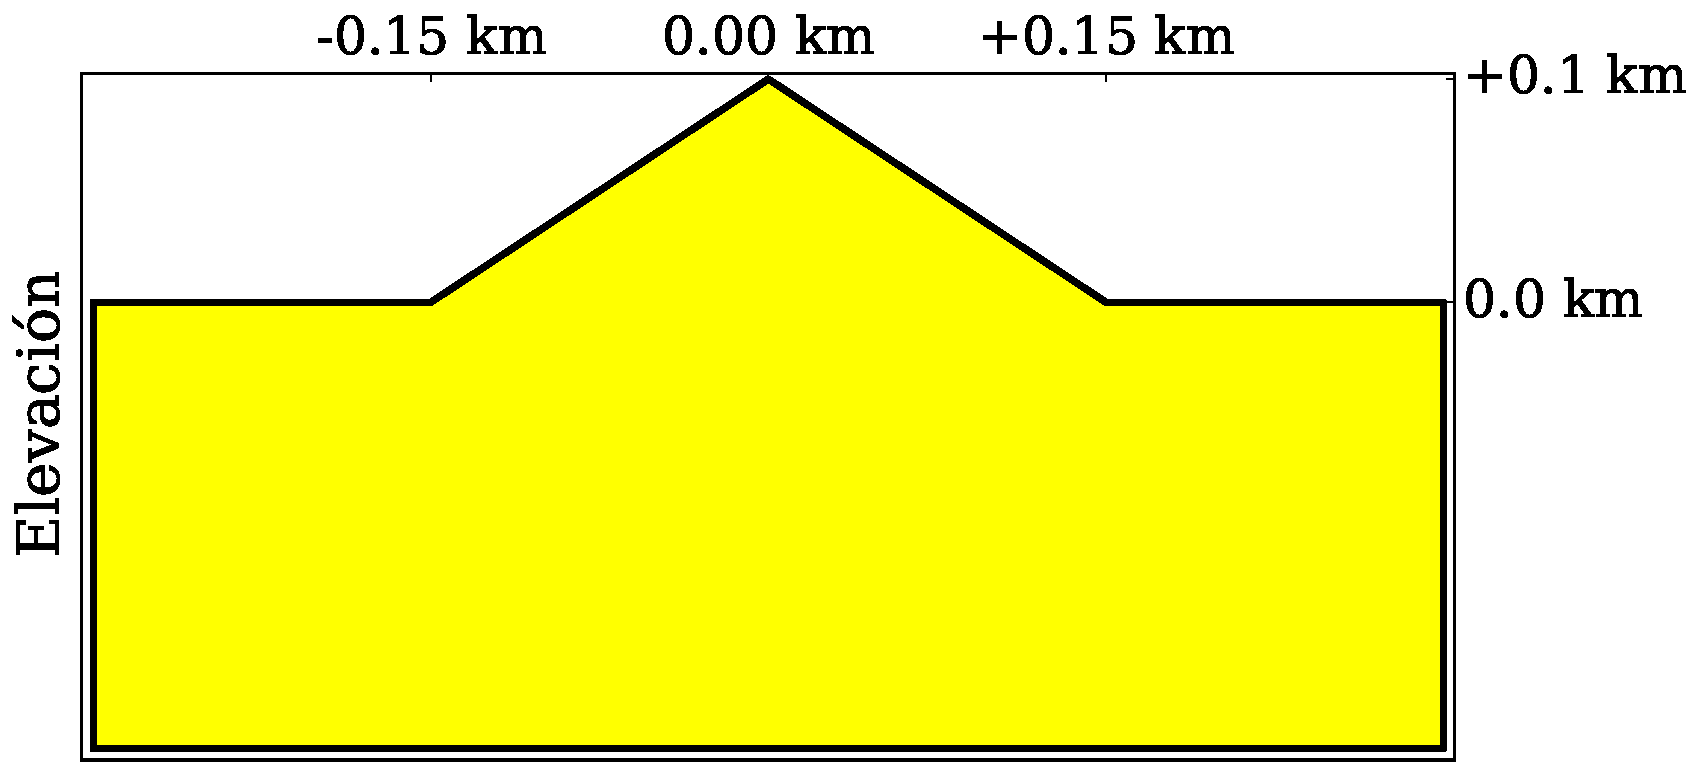
\includegraphics[width=8 cm]{img/ModelLocal.pdf}}
	%
	\subfloat [Modelo Regional]{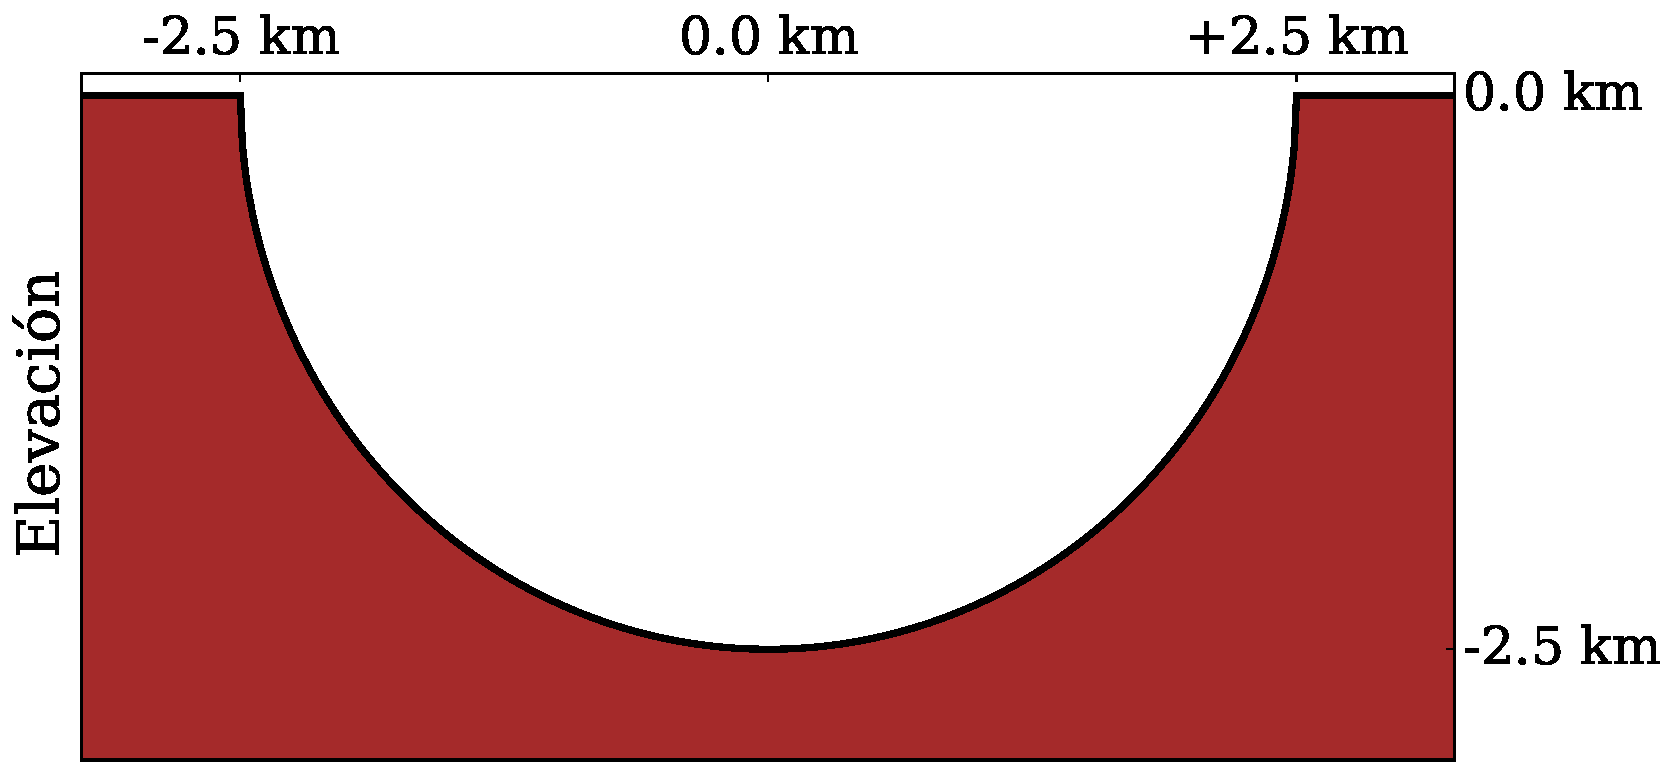
\includegraphics[width=8 cm]{img/ModelRegional.pdf}}
	\vspace{-.5 cm}
    \caption{Modelo local y regional.}
    \label{fig:modellocalregional}
    \vspace{-1 cm}
\end{figure}

La figura \ref{fig:modellocalregional} muestras dos geometrías con diferente orden de escala. La figura \ref{fig:modellocalregional}a corresponde al modelo de un dispersor tipo montaña, el cual dadas sus dimensiones, lo denominaremos \textit{Modelo Local} y al dispersor de la figura \ref{fig:modellocalregional}b, el cual corresponde a un cañón semicircular de radio $r=2.5\ km$, lo denominaremos \textit{Modelo Regional}. Ambos modelos son lineales, elásticos y homogéneos, con velocidad de propagación y densidad unitarias y se excitan con ondas de corte tipo \textit{SH}.

\subsection{Respuesta Local}

La respuesta local corresponde a la generada por topografías con dimensiones menores o iguales a $\ell$, geometría que no perturba la respuesta para longitudes de onda mucho mayores a dicha dimensión $\left( \lambda \gg \ell \right)$, dónde $\lambda$ es la longitud de onda, o que la perturbación que éstas generan en la respuesta es tan pequeña que es posible despreciarla.

\begin{figure}[H]
	\centering
	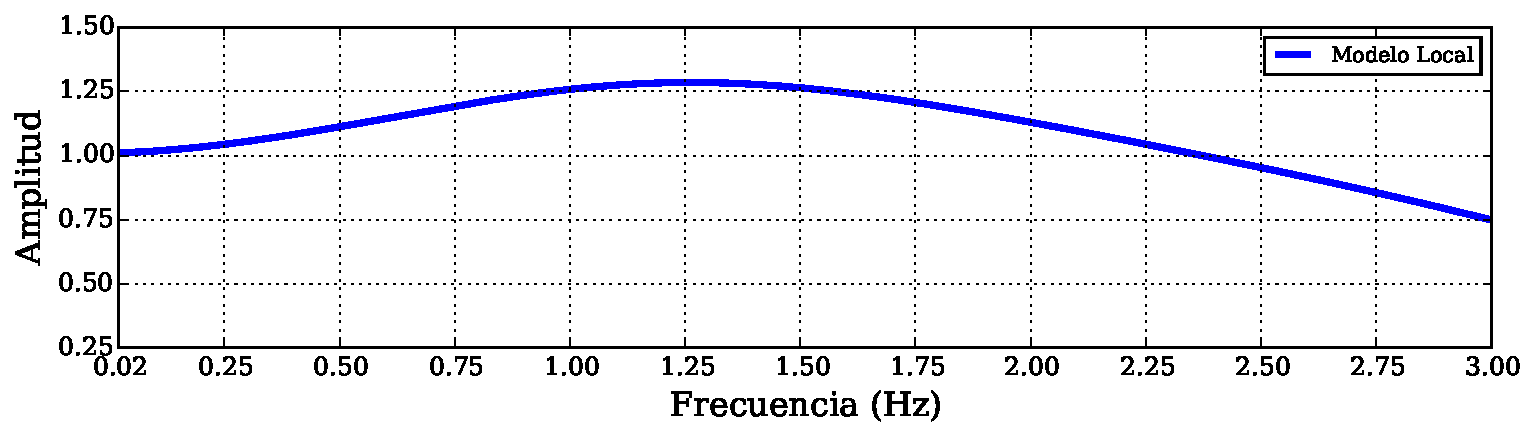
\includegraphics[width=15.5 cm]{img/LocalResponse.pdf}
	\vspace{-1 cm}	
	\caption{Función de Transferencia Modelo Local, Mitad Talud Izquierdo}
	\label{fig:localresponse}
	\vspace{-.5 cm}
\end{figure}

En la figura \ref{fig:localresponse} se presenta la función de transferencia sobre la mitad del talud izquierdo del dispersor de la figura \ref{fig:modellocalregional}a. En dicha figura se observa como para un rango de frecuencias bajo, longitud de onda mucho mayor que la base de la montaña analizada $\left( \lambda \gg base \right)$, la función de transferencia es muy cercana a la unidad $\left( FT\sim 1.0 \right)$, lo cual quiere decir que dicho dispersor no modifica, o lo hace muy poco, la respuesta. Es precisamente para dispersores con dimensiones que no exciten dichos rangos de frecuencias, que definiremos la \textit{Respuesta Local}.

\subsection{Respuesta Regional}

La respuesta regional corresponde a la generada por topografías con dimensiones mayores a $L$, dimensión que no modifica la respuesta para longitudes de onda lo suficientemente pequeñas $\left( \lambda \ll L \right)$ ya que éstas verán la geometría como un semiespacio y por tanto la función de transferencia tiende a la unidad $\left( FT \sim 1.0 \right)$.

\begin{figure}[H]
	\centering
	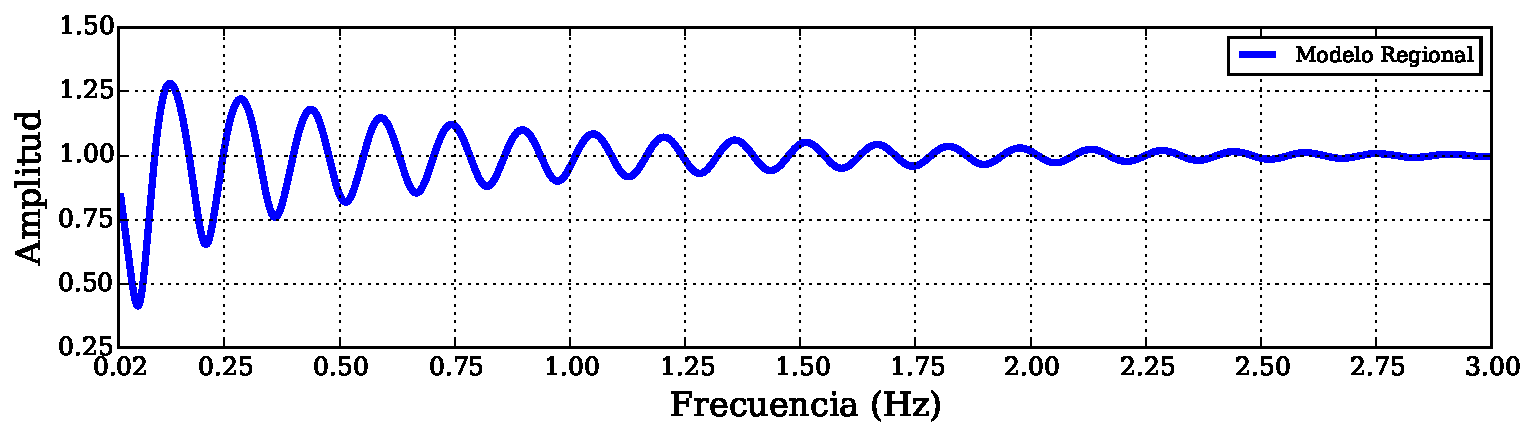
\includegraphics[width=15.5 cm]{img/RegionalResponse.pdf}
	\vspace{-1 cm}
	\caption{Función de Transferencia Modelo Regional Fondo del Cañón}
	\label{fig:regionalresponse}
	\vspace{-1 cm}
\end{figure}

En la figura \ref{fig:regionalresponse} se presenta la función de transferencia para un punto ubicado en el fondo del cañón semicircular del modelo regional, figura \ref{fig:modellocalregional}b. En dicha figura se observa como en la baja frecuencia, longitudes de onda grandes, la respuesta se aleja bastante de la unidad, algunas veces amplificandose la respuesta y en otras deamplificandose, pero a partir de un rango de frecuencias determinado, la respuesta comienza a oscilar muy cerca de la unidad hasta que dicha oscilación parece desvanecerse del todo. Este tipo de respuestas, o geometrías a gran escala, serán las que denominamos \textit{Respuesta Regional} ya que no modifica, o lo hace muy poco, la respuesta en la alta frecuencia.
%
%
%
%
%
\section{Objetivos}
%
\subsection{Objetivo General}
%
Estudiar la respuesta de la topografía regional y considerar su efecto sobre las topografías locales para la realización de estudios de efectos de sitio unidimensionales $\left(1D\right)$, bidimensionales $\left(2D\right)$ y tridimensionales $\left(3D\right)$.
%
\subsection{Objetivos Específicos}
%
\begin{itemize}
%
	\item Demostrar que la respuesta total de un sitio particular se puede construir a partir de una correspondiente a la baja frecuencia, respuesta regional, y otro en la alta frecuencia, respuesta local.
	%
	\item Demostrar la importancia de la respuesta regional en la respuesta de una geometría local.
	%
	\item Determinar el efecto topográfico regional de una región específica e incluir su efecto en la respuesta sísmica local de un sitio particular.
	%
	\item Proponer una metodología para la elaboración de estudios de microzonificación sísmica considerando el efecto regional de la topografía y el efecto local acoplado suelo-topografía.
	%
	\item Tomando como base una microzonificación sísmica ficticia o existente, elaborada con los modelos tradicionales $1D$ de propagación de ondas, comparar los resultados versus la metodología propuesta para modelos $1D$, $2D$ y $3D$ de propagación de ondas.
%
\end{itemize}
%
%
%
%
%
\section{Marco Conceptual}
%
Los efectos de sitio consisten en la determinación de los movimientos del suelo de un sitio particular en términos de espectros de respuesta para ser usados en el diseño sismoresistente de estructuras. A pesar de que existe fuerte evidencia teórica, numérica y experimental de que éste problema depende fuertemente del tipo de onda incidente, de las propiedades mecánicas de los suelos presentes y de la topografía superficial y sub-superficial \citep[por ejemplo en][]{Assimaki2013, Ashford1997, Aki1993, Barani2014}, los procedimientos actuales solo consideran el efecto mecánico en la respuesta mediante el análisis de modelos $1D$ de propagación de ondas  y las normas de diseño y construcción sismoresistente solo introducen factores de modificación espectral que se usan para modificar los espectros de diseño en función de la velocidad de propagación de los suelos locales.\\
%
Adicionalmente, la respuesta local puede verse afectada no solo por la topografía local y la estratigrafía sino también por la topografía regional o de gran escala dentro de la cual se encuentre el sitio particular. La consideración de los efectos regionales o de gran escala representan un problema bastante complejo que demanda altos recursos computacionales, con los cuales solo cuentan unos cuantos grupos de investigación al rededor del mundo \citep[ver][]{Doriam2014, Graves2011} y su uso aún se encuentra muy lejos de la práctica profesional.

Teóricamente el problema de los efectos de sitio generados por la topografía puede ser abordado mediante el uso de factores de agravamiento topográfico, donde éstos factores se aplican directamente sobre los espectros generados a partir del análisis de modelos de propagación $1D$ de ondas. Los factores de agravamiento topográfico no han sido implementados en las normas de diseño sismoresistentes tal véz debido a lo difícil de su parametrización en funciones simples. Por lo anterior, la consideranción de los efectos topográficos considerando todos los factores que afectan la respuesta parece estar limitada al uso de modelos computacionales a gran escala altamente elaborados con técnicas numéricas como el método de los elementos finitos, el método de los elementos finitos espectrales o el método de las diferencias finitas.

En la siguiente sección presentaremos una propuesta metodológica para el estudio de los efectos de sitio, la cual puede ser incorporada en la práctica profesional. En ésta propuesta se construye un modelo computacional local, regional y completo de unas geometrías altamente idealizadas. Los resultados de la geometría regional se usarán para modificar la respuesta local y así obtener la respuesta total combinando las dos anteriores y a su vez compararla con la respuesta del modelo completo.

La idea fundamental de ésta propuesta es que la topografía regional puede ser parametrizada en unos factores simples o puede ser estudiada por medio de modelos altamente simplificados y con éstos modificar las señales de excitación de modelos locales altamente detallados, en los cuales se pueden considerar los modelos constitutivos de los suelos y su comportamiento en el rango no-lineal.
%
%
%
%
%
\section{Metodología}
%
Las hipótesis fundamentales en las cuales se basa éste trabajo, y que deberán ser probadas, consisten en:
%
\begin{itemize}
%
	\item Los efectos de fuente y ruta de propagación se encuentran incluidos en los espectros de amenaza sísmica uniforme, los cuales se construyen a partir de los registros de sismos reales y la sismología regional.
	%
	\item La respuesta sísmica de un sitio específico es posible obtenerla como la superposición de una respuesta en la baja frecuencia, \textit{Respuesta Regional}, y una respusta en la alta frecuencia, \textit{Respuesta Local}.
	%
	\vspace{-.5 cm}
%
\end{itemize}
%
La metodología propuesta consiste en construir la respuesta total de un sitio particular como la superposición de una respuesta regional, debida a la topografía regional o de gran escala, y una respuesta local o de menor escala, debida a la topografía local y la estratigrafía del sitio. La respuesta local será calculada a partir de modelos semi-analíticos o con simulaciones que solo capturen la respuesta en la baja frecuencia, ya que en la alta frecuencia la respuesta debe acercarse bastante a la de un semiespacio. La respuesta local se obtendrá a partir de simulaciones altamente detalladas usando modelos computacionales con elementos finitos, asumiendo que éstos se encuentran soportados sobre un semi-espacio lineal elástico, pero pudiendose considerar el comportamiento no-lineal de los diferentes materiales locales. Los modelos computacionales por elementos finitos se excitarán usando los procedimientos convencionales para los modelos unidimensionales $\left( 1D \right)$ de propagación de ondas; en los cuales un espectro de amenaza sísmica uniforme se convierte en una familia de acelerogramas sintéticos en roca, los cuales deben representar sismos generados por fuentes ubicadas a diferentes distancias de la región de estudio. A los acelerogramas sintéticos se les calculará los espectros de Fourier para modificarlos con las funciones de transferencia de la respuesta regional y nuevamente se llevarán al dominio del tiempo para tener así unos acelerogramas sintéticos que incluyan el efecto de la respuesta regional. Estos acelerogramas sintéticos modificados por el efecto regional se aplicarán como excitación de los modelos computacionales del sitio, inicialmente en foma de ondas planas tipo $SH$ y $SV$ incidiendo verticalmente, y por último empleando modelos tridimensionales $\left( 3D \right)$.\\
%
Para el análisis de los modelos locales se desarrollará una herramienta computacional, la cual permitirá considerar el efecto acoplado suelo-topografía en el rango lineal y no-lineal. La herramienta computacional ha desarrollar se encuentra basada en el método del dominio reducido, DRM por sus siglas en inglés, presentado por \citeauthor{bielak2003} (\citeyear{bielak2003}) para poder incluir los efectos de fuente en simulaciones a gran escala sobre escenarios reales. En nuestro trabajo utilizaremos una versión modifcada del DRM ya que primero calculamos la respuesta sin la topografía local, respuesta que usamos para modificar la excitación de los modelos locales.

A continuación se presenta una descripción detallada de nuestra metodología, la cual según el conocimiento de los autores de ésta propuesta no ha sido presentada antes:

Partiendo del espectro de amenaza uniforme \begin{large} $S_{a}^{UH} \left( T \right)$ \end{large}, el cual se calcula en roca y se encuentra libre de efectos mecánicos y topogáficos, es posible generar historias de aceleraciones sintéticas \begin{large} $a_{i}^{UH}\left( t \right)$ \end{large}. Es necesario generar varias señales, las cuales deben ser representativas de sismos ocurridos a diferentes distancias del sitio bajo estudio, donde cada señal genera un espectro de respuesta $S_{a}^{i} \left( T \right)$ diferente al de amenaza uniforme pero los cuales se encuentran contenidos dentro de éste.

\begin{large}
	$S_{a}^{UH} \left( T \right) \Rightarrow a_{i}^{UH}\left( t \right) \Rightarrow S_{a}^{i} \left( T \right)$
\end{large}

Donde $S_{a}^{UH} \left( T \right)$ corresponde al espectro de respuesta de amenaza uniforme, $a_{i}^{UH}\left( t \right)$ $i$-esima señal sintética generada a partir del espectro de amenaza uniforme y $S_{a}^{i} \left( T \right)$ al espectro de respuesta de la $i$-esima señal sintética. Además se tiene que:
%
\begin{large}
	\begin{align}
		S_{a}^{1} \left( T \right) \cup S_{a}^{2} \left( T \right) \cup S_{a}^{3} \left( T \right) \cup ... \cup S_{a}^{n} \left( T \right) = S_{a}^{UH} \left( T \right)
		\vspace{-1 cm}
	\end{align}	
\end{large}
%
%
De las señales sintéticas es posible calcular el espectro de Fourier de cada una de ellas, teniendo en cuenta que éstas contienen el campo incidente y el reflejado:
%
\begin{large}
	\begin{align}\label{eq:espfouhs}
		\widehat{A}^{HS}_{i} \left( \hat{i} \omega \right) = \dfrac{1}{2} \widehat{A}^{FS}_{i} \left( \hat{i} \omega \right)
	\vspace{-1 cm}
	\end{align}
\end{large}
%
Donde $\widehat{A}^{FS}_{i} \left( \hat{i} \omega \right)$ corresponde al espectro de Fourier de la $i$-esima señal sintética, incluye el campo incidente y el reflejado, $\widehat{A}^{HS}_{i} \left( \hat{i} \omega \right)$ es el espectro de Fourier de la $i$-esima señal sintética, solo incluye el campo incidente.\\
%
El espectro de Fourier de la $i$-esima señal sintética se define como:
%
\begin{large}
	\begin{align}\label{eq:fourdirec}
		\widehat{A}^{FS}_{i} \left( \hat{i} \omega \right) = \int_{-\infty}^{+\infty} a_{i}^{UH} \left( t \right) e^{-\hat{i} \omega t} dt 
	\vspace{-1 cm}
	\end{align}
\end{large}
%
El proceso anterior se puede resumir en el siguiente esquema:

\begin{large}
	$a_{i}^{UH}\left( t \right) \Rightarrow \widehat{A}^{FS}_{i} \left( \hat{i} \omega \right) \Rightarrow \widehat{A}^{HS}_{i} \left( \hat{i} \omega \right)$
\end{large} 

La región bajo estudio se aproxima a una geometría sencilla, la cual puede ser posible estudiarla mediante procedimientos semi-analíticos o con simulaciones que solo incluyen la respuesta lineal en la baja frecuencia. En la figura \ref{fig:geolocreg} se presenta un ejemplo hipotético de una geometría regional en conjunto con la geometría aproximada; la geometría regional se muestran algunas geometrías locales y la presencia de diferentes materiales. En la geometría aproximada se ha homogeneizado el dominio.

\begin{figure}[H]
	\centering
	\subfloat [Geometría Regional]{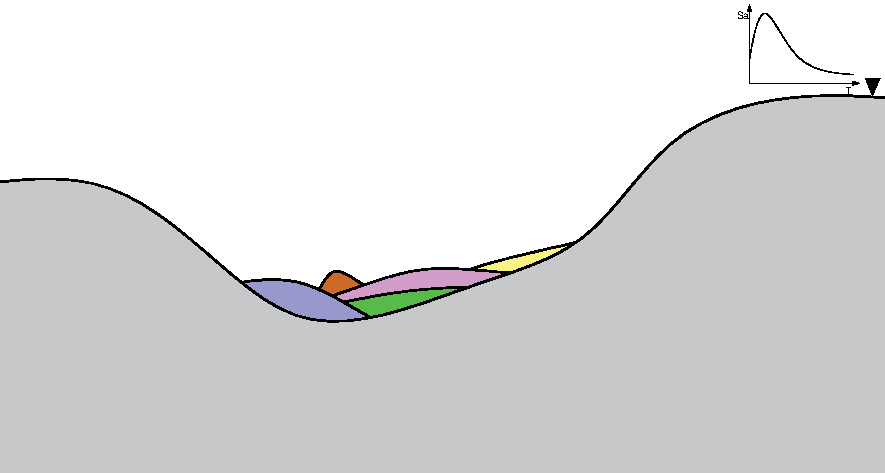
\includegraphics[width=7.5 cm]{img/Regional.pdf}}
	\hspace{.25 cm}
	\subfloat [Geometría Regional Aproximada]{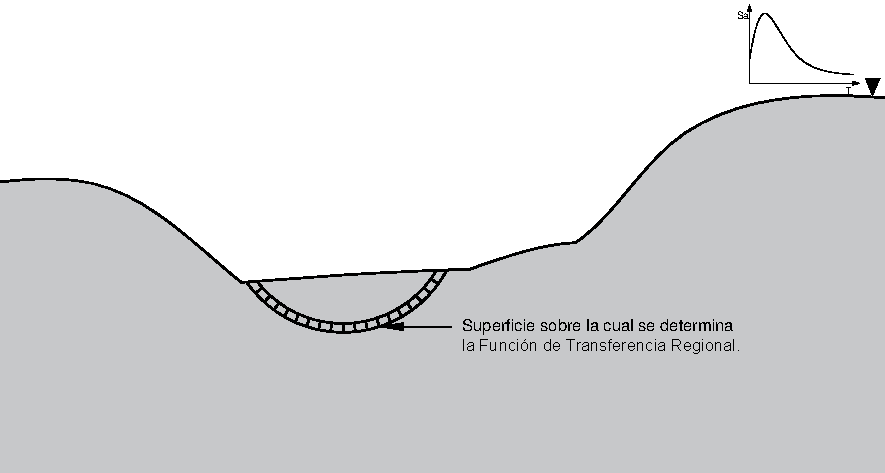
\includegraphics[width=7.5 cm]{img/FunTrans.pdf}}
	\vspace{-.5 cm}
    \caption{Geometría Regional.}
    \label{fig:geolocreg}
    \vspace{-1 cm}
\end{figure}
%

La respuesta de la geometría regional de la figura \ref{fig:geolocreg}b, en términos de funciones de transferencia $FT^{Ref} \left(\hat{i} \omega \right)$, se emplea para modificar los espectros de Fourier de las señales sintéticas.
%
\begin{large}
	\begin{align}\label{eq:espfoumod}
		\widehat{A}^{Mod}_{i} \left( \hat{i} \omega \right) = \widehat{A}^{HS}_{i} \left( \hat{i} \omega \right) FT^{Ref} \left( \hat{i} \omega \right)
	\vspace{-1 cm}
	\end{align}
\end{large}
%
Donde $\widehat{A}^{Mod}_{i} \left( \hat{i} \omega \right)$ corresponde al espectro de Fourier modificado por el efecto de la topografía regional. A partir del espectro de Fourier modificado se calculan las nuevas señales sintéticas vía la transformada inversa de Fourier, señales que se emplean para excitar los modelos locales.
%
\begin{large}
	\begin{align}\label{eq:fourinv}
		a_{i}^{Mod} \left( t \right) = \dfrac{1}{2 \pi} \int_{-\infty}^{+\infty} \widehat{A}^{Mod}_{i} \left( \hat{i} \omega \right) e^{\hat{i} \omega t} d \omega
	\vspace{-1 cm}
	\end{align}
\end{large}
%
El proceso anterior se puede resumir en el siguiente esquema:

\begin{large}
	$FT^{Ref} \left( \hat{i} \omega \right) \Rightarrow \widehat{A}^{Mod}_{i} \left( \hat{i} \omega \right) \Rightarrow a_{i}^{Mod}\left( t \right)$
\end{large}

Las señales sintéticas modificadas $a_{i}^{Mod}\left( t \right)$ se emplean para excitar los modelos locales, los cuales incluyen la topografía superficial y sub-superficial. La necesidad de considerar sismos que representen fuentes ubicadas a diferentes distancias del sitio de estudio se debe a que es necesario estudiar la respuesta lineal y no-lineal de los modelos.

\begin{figure}[H]
	\centering
	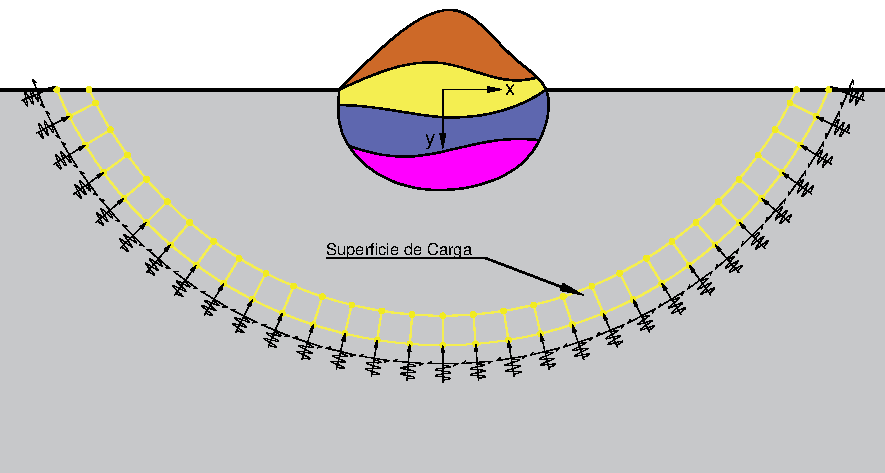
\includegraphics[width=12 cm]{img/Local.pdf}
	\vspace{-.5 cm}
	\caption{Modelo Local}
	\label{fig:local}
	\vspace{-1 cm}
\end{figure}
%
En la figura \ref{fig:local} se presenta el esquema de un modelo local, el cual contiene topografía superficial y subsuperficial, presencia de diferentes materiales, sobre un semiespacio homogéneo junto con la superficie sobre la cual se aplica la excitación modificada por los efectos regionales.

El análisis de los modelos locales es el encargado de capturar la respuesta en la alta frecuencia, respuesta generada por la topografía y el efecto mecánico local; el efecto acoplado suelo-topografía. La formulación aquí presentada es diferente a la original del DRM presentada por \citeauthor{bielak2003} (\citeyear{bielak2003}) ya que en la primer etapa calculamos la respuesta regional sin la topografía ni materiales locales, respuesta que posteriormente modifica el campo incidente y se aplica como una carga efectiva como se muestra en la figura \ref{fig:local}. El método para excitar los modelos locales se implementará en software comercial por elementos finitos de manera que pueda ser usado fácilmente en los estudios de efectos de sitio.

La respuesta de los modelos computacionales locales, en términos de aceleraciones, se usarán para calcular los espectros de respuesta totales $S_{a}^{Tot} \left( T \right)$, los cuales consideran los efectos de fuente y ruta de progagación, al ser éstos excitados con señales sintéticas generadas a partir de espectros de amenaza uniforme $S_{a}^{UH} \left( T \right)$, el efecto de la topografía regional con la consideración de la función de transferencia regional $FT^{Ref} \left( \hat{i} \omega \right)$, y la respuesta lineal y no-lineal del efecto acoplado suelo topografía local.\\
%
Los espectros de respuesta totales $S_{a}^{i-Tot} \left( T \right)$, para cada una de las señales sintéticas y sobre toda la superficie del dominio, se usarán para calcular la relación de respuesta espectral, la cual se usa para modificar el espectro de amenaza uniforme por el efecto regional y acoplado suelo-topografía local.
%
\begin{large}
	\begin{align}\label{eq:rrs}
		\mathcal{RRS}^{i} \left( T \right) = \dfrac{S_{a}^{i-Tot} \left( T \right)}{S_{a}^{i} \left( T \right)}
	\vspace{-1 cm}
	\end{align}
\end{large}
%
\begin{large}
	\begin{align}\label{eq:rrs}
		S_{a}^{UH-Mod} \left( T \right) = S_{a}^{UH} \left( T \right) * envol\left\lbrace \mathcal{RRS}^{i} \left( T \right) \right\rbrace
	\vspace{-1 cm}
	\end{align}
\end{large}
%
Donde $S_{a}^{UH-Mod} \left( T \right)$ corresponde al espectro de amenaza uniforme modificado por el efecto regional y local, $envol \left\lbrace \mathcal{RRS}^{i} \left( T \right) \right\rbrace$ corresponde a la envolvente de las relaciones de respuestas espectrales.
%
%
%
%
%
\section{Resultados Preliminares}
%
La metodología propuesta se emplea para analizar un modelo simplificado sobre el que se incide verticalmente una onda plana tipo $SH$. Para el análisis de los modelos regionales y locales se utiliza un programa computacional de Elementos de Frontera 2D (BEM por sus siglas en inglés) desarrollado al interior del grupo de Mecánica Aplicada de la Universidad EAFIT (Medellín, Colombia), el cual encuentra la respuesta en el dominio de la frecuencia y por lo tanto los resultados se limitarán, en esta propuesta, al rango lineal. Todos lo cálculos fueron realizados en el computador de alto desempeño Apolo de la Universidad EAFIT.
%
\begin{figure}[H]
	\centering
	\subfloat [Modelo Completo]{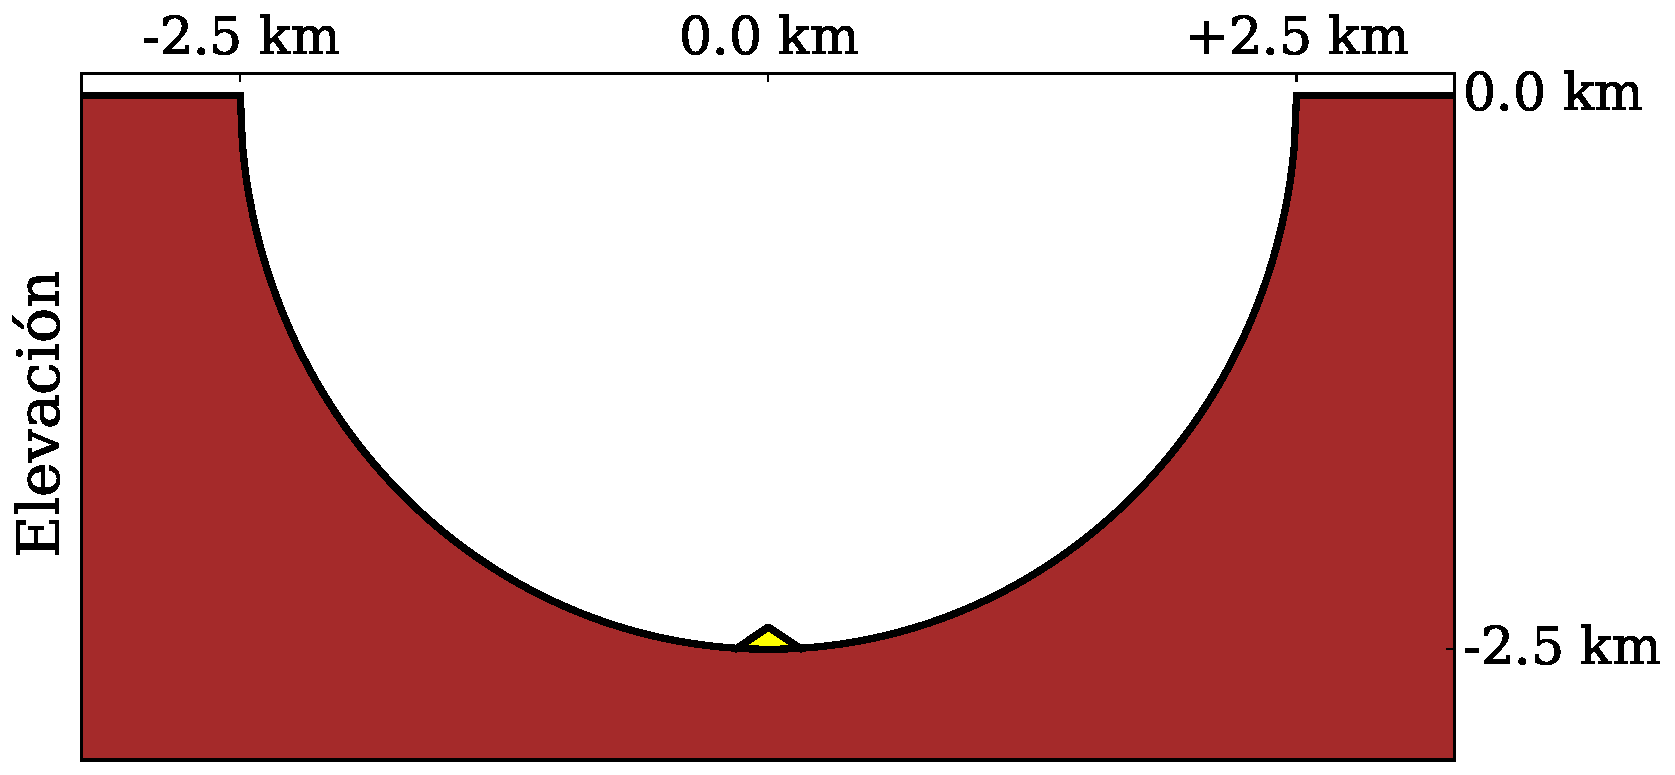
\includegraphics[width=16 cm]{img/ModelRegionalComplete.pdf}}\\
	%
	\subfloat [Modelo Local]{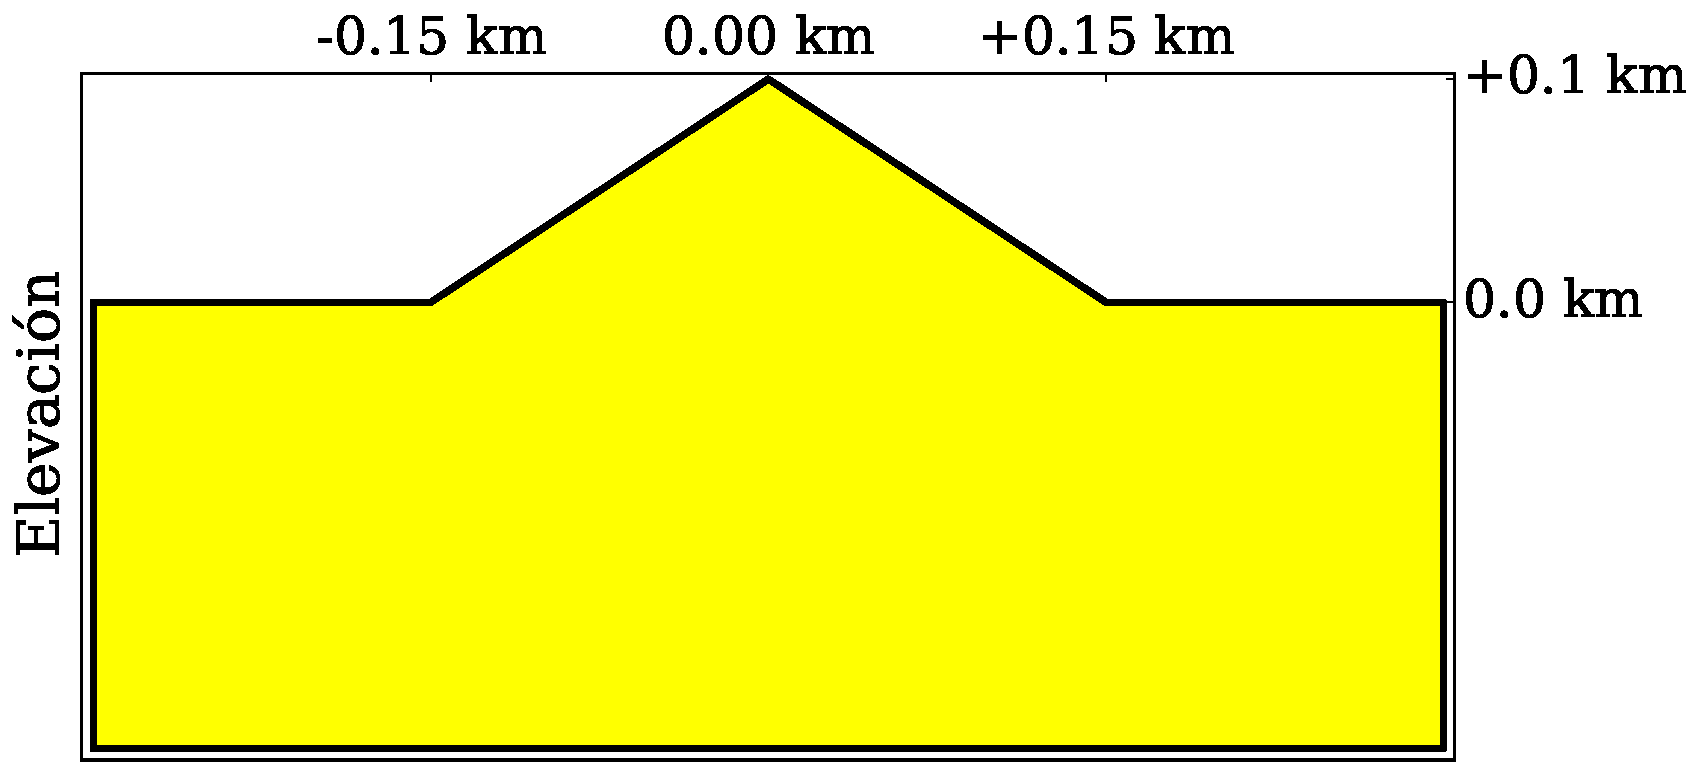
\includegraphics[width=8 cm]{img/ModelLocal.pdf}}
	%
	\subfloat [Modelo Regional]{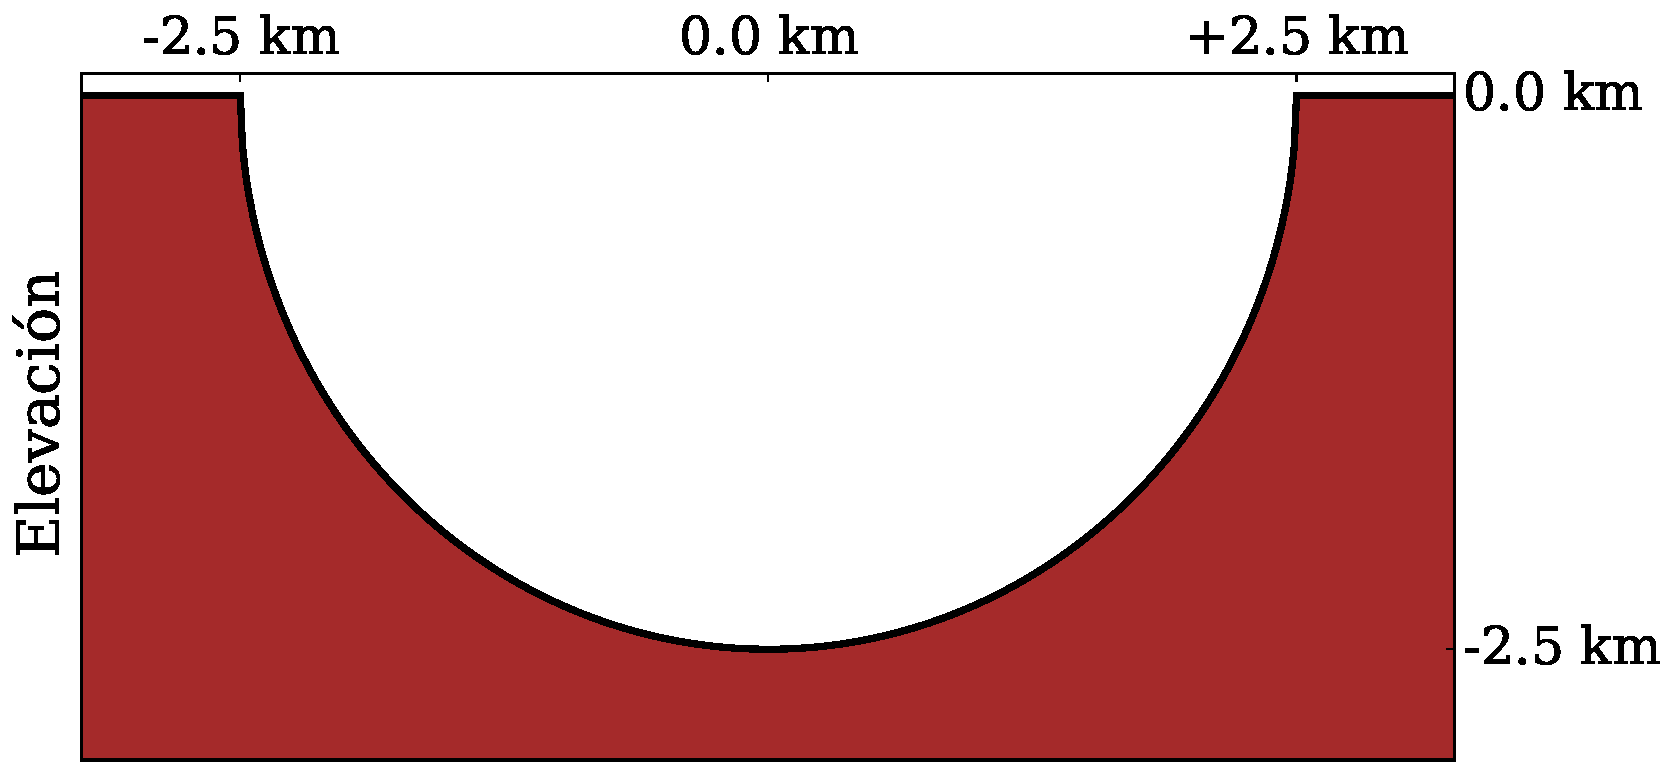
\includegraphics[width=8 cm]{img/ModelRegional.pdf}}
	\vspace{-.5 cm}
    \caption{Modelo 1.}
    \label{fig:model1}
    \vspace{-.5 cm}
\end{figure}
%
Inicialmente se analiza un modelo en el cual tanto la geometría regional como local tienen las mismas propiedades, modelo homogéneo. En el segundo modelo, la velocidad de propagación del material del dispersor local se definirá igual a la mitad del semiespacio.

En la figura \ref{fig:model1} se presentan los tres modelos analizados. La figura \ref{fig:model1}a corresponde al modelo completo, el cual contiene la topografía regional y local; la respuesta de éste modelo será usada para verificar la eficiencia del método. La figura \ref{fig:model1}b corresponde al modelo de la topografía local, en éste se asume que ésta se encuentra sobre un semiespacio homogéneo en el cual la única irregularidad corresponde a la montaña, por lo tanto se desprecia la interacción entre la topografía local y la toporgrafía regional. La figura \ref{fig:model1}c corresponde al modelo de la topografía regional en el cual se asume un medio homogeneo y se ha eliminado la topografía local quedando un semicirculo, en éste modelo se desprecia la interacción entre la respuesta de la montaña y la geometría regional. %Adicionalmente se analizarán modelos de propagación unidimensional, para el modelo en el cual la montaña tiene una velocidad de propagación diferente, en los cuales se tomará la altura del estrato igual a la profundidad del punto donde se evalúa la respuesta. ESTO AÚN LO DEBO PROCESAR BIEN PARA PODER METERLO ACÁ, ADEMÁS NO ENTIENDO BIEN LOS RESULTADOS QUE ME ESTÁN DANDO.

En la figura \ref{fig:puntos} se muestra un ``zoom" de la montaña dentro del modelo completo. En ésta se muestran los puntos en los cuales se presenta la respuesta. Dentro del modelo regional, los puntos en los cuales se evalúa la respuesta corresponden a la proyección de los de la superficie de la montaña.

\begin{figure}[H]
	\centering
	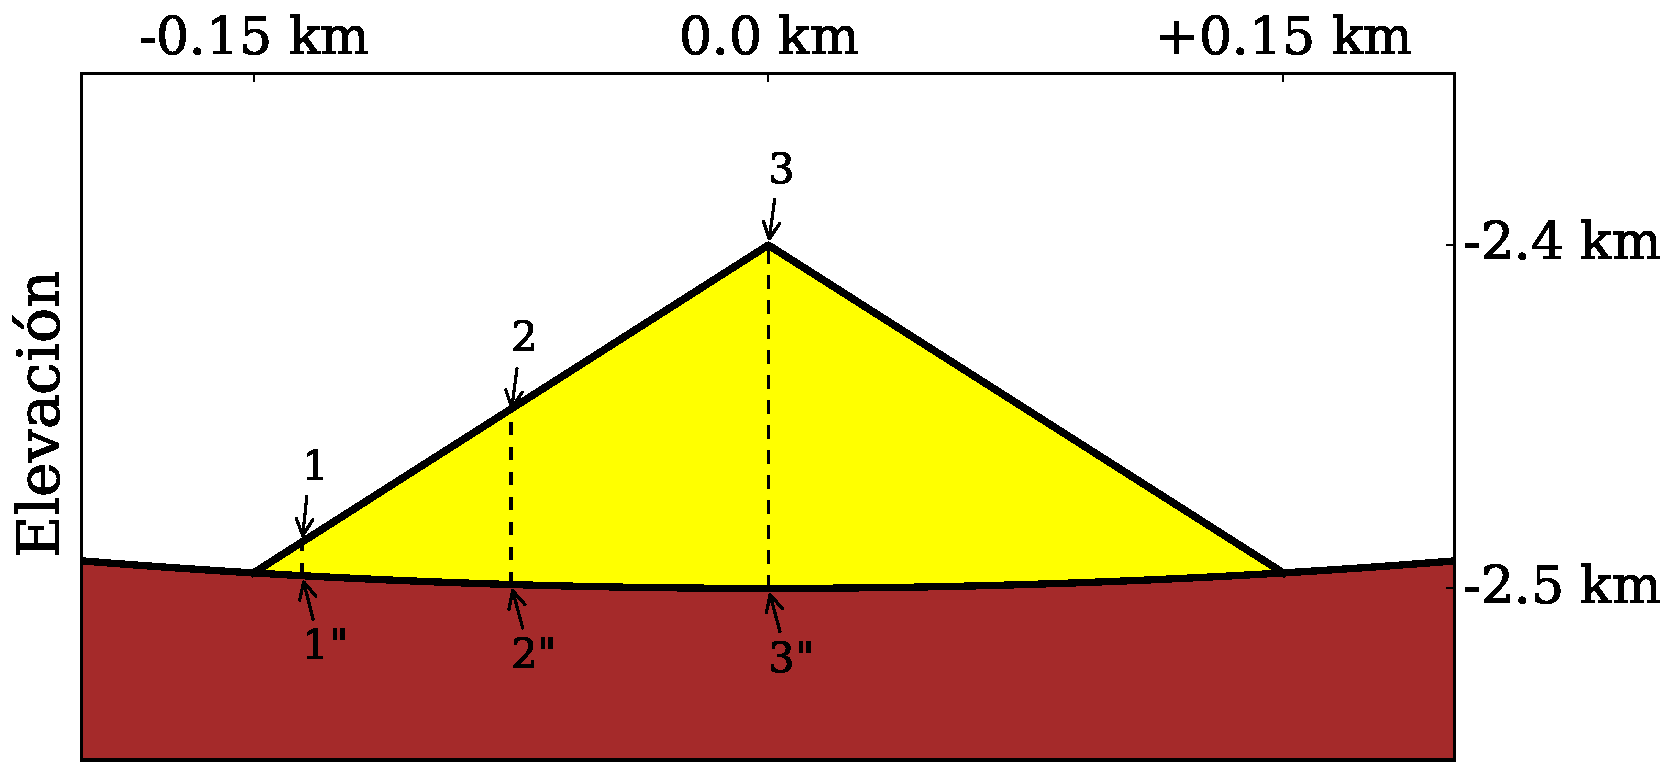
\includegraphics[width=12 cm]{img/ModelRegionalCompleteZoom.pdf}
	\vspace{-.5 cm}
	\caption{Puntos Evaluación Respuesta}
	\label{fig:puntos}
	\vspace{-1 cm}
\end{figure}
%

Los puntos sobre la superficie de la montaña se numeran como:
%
\begin{itemize}
%
	\item $1$: Esquina izquierda de la montaña.
	\item $2$: Mitad de la ladera.
	\item $3$: Vértice Superior
	\vspace{-.5 cm}
%
\end{itemize} 

La proyección sobre el fondo del modelo regional se numeran como $1"$, $2"$ y $3"$.

Adicional a la respuesta de los tres modelos se presentará la respuesta del \textbf{\textit{``Modelo Local Modificado"}}, la cual se encuentra multiplicando la función de transferencia del modelo local por la del modelo regional.
%
\begin{large}
	\begin{align}
		FT^{MLM} \left(\hat{i} \omega \right)= FT^{MR} \left(\hat{i} \omega \right) * FT^{ML} \left(\hat{i} \omega \right) 
		\vspace{-1 cm}
	\end{align}
\end{large}
%
$FT^{MLM} \left(\hat{i} \omega \right)$ corresponde a la función de transferencia del modelo modificado, $FT^{MR} \left(\hat{i} \omega \right)$ es la función de transferencia del modelo regional y $FT^{ML} \left(\hat{i} \omega \right)$ la función de transferencia del modelo local.

Los elementos de los tres modelos se dimensionan según la \cref{eq:tamelem}:
%
\begin{large}
	\begin{align}\label{eq:tamelem}
		\ell_{max} = \dfrac{\beta_{min}}{p * f_{max}}
 	\end{align}
\end{large}
%
Donde $\ell_{max}$ corresponde al tamaño máximo de los elementos y $p$ corresponde al número de puntos por longitud de onda.
%
\subsection{Montaña Triangular Embebida en un Sector Semi-Circular, Modelo Homogéneo}
%
Para los tres modelos analizados se emplea la misma velocidad de onda de corte $\beta = 1.0\ km/s$, densidad $\rho = 1000\ kg/m^3$ y frecuencia máxima $f_{max} =  16\ Hz$. El sector semicircular tiene un radio $r=2.50\ km$, la montaña una base $b=0.30\ km$ y altura $h=0.10\ km$.

Para los tres modelos se emplean $24$ puntos por longitud de onda $\left( p = 24 \right)$.

En la figura \ref{fig:ftspatial} se muestran las funciones de transferencia sobre la superficie de los tres modelos de la figura \ref{fig:model1}, entre las coordenadas $-0.15\ km$ y $+0.15\ km$.\\
%
En la \cref{fig:ftspatial}a, la cual corresponde a una frecuencia igual a $0.20\ Hz$, no se observa variación espacial de la respuesta debido a que la longitud de onda es mucho mayor que la longitud sobre la cual se obser va la respuesta. La respuesta del modelo local de la figura \ref{fig:model1}b tiende a la de un semiespacio, debido a que la longitud de onda es aproximadamente $17$ veces el ancho de la base de la montaña, $\lambda= 5.0\ km$, y la respuesta no ve el dispersor; por ésta misma razón, la respuesta del modelo regional y la del modelo completo son iguales.
%
\begin{figure}[H]
	\centering
	\subfloat []{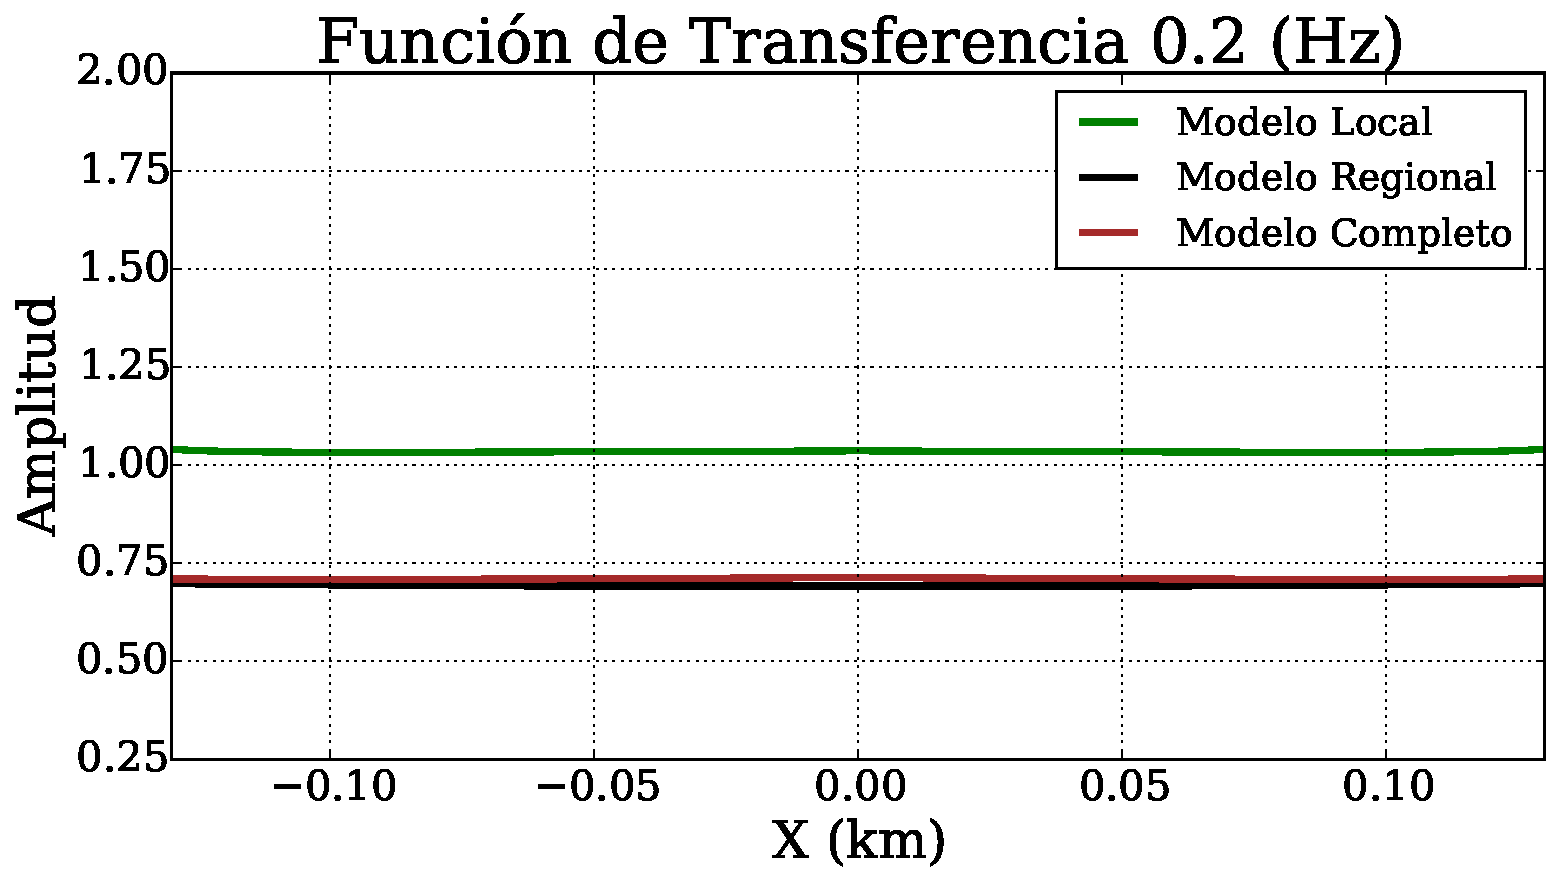
\includegraphics[width=8 cm]{img/TF_Homogeneo_2.pdf}}
	\subfloat []{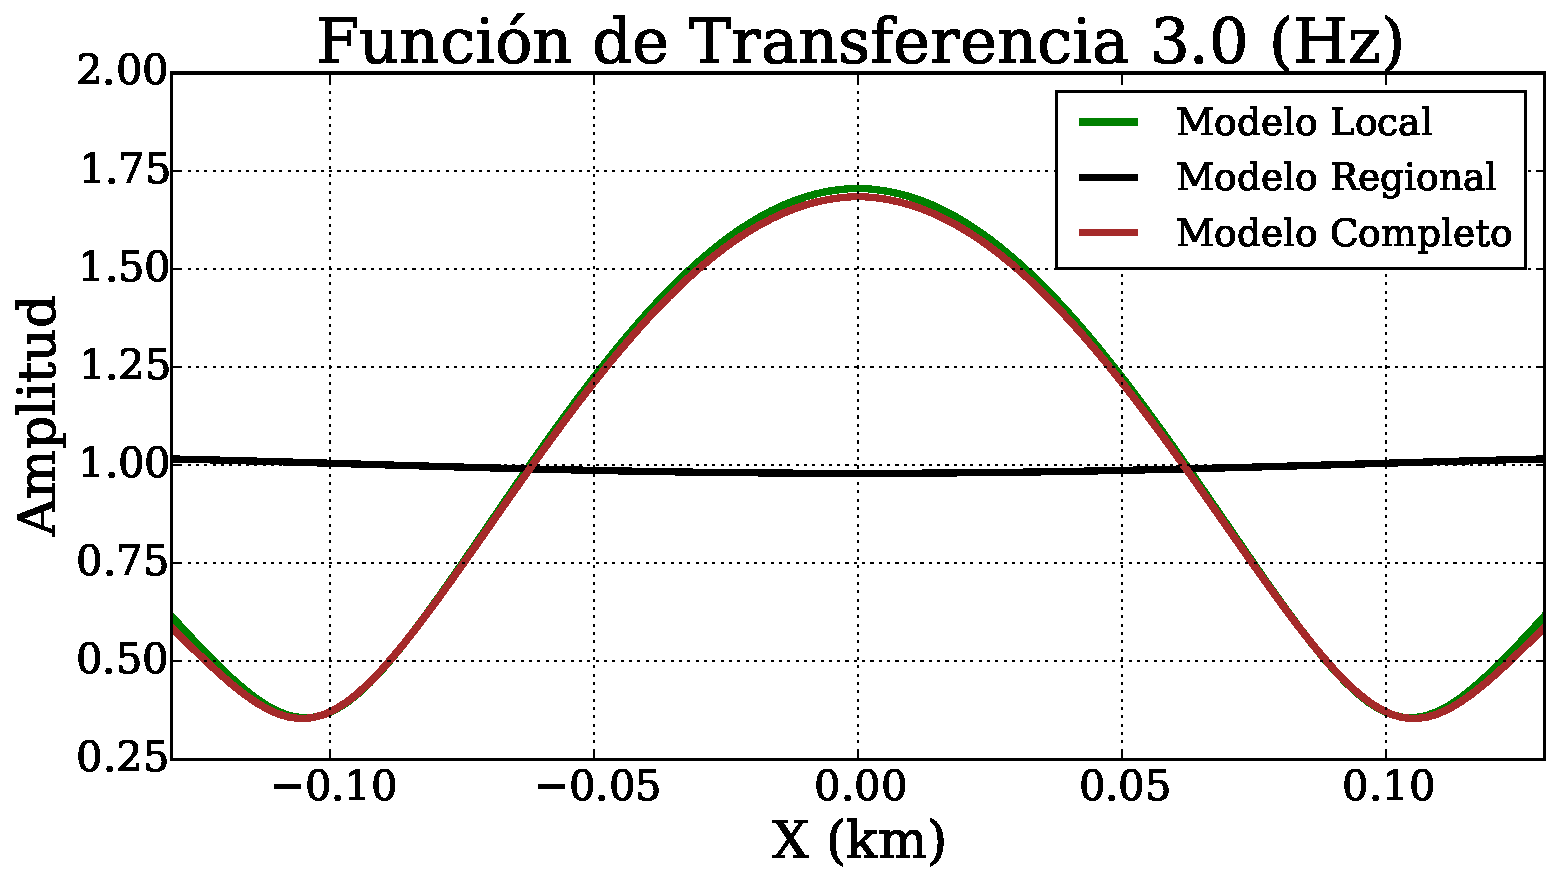
\includegraphics[width=8 cm]{img/TF_Homogeneo_30.pdf}}\\
	\vspace{-.5 cm}
	%
    \caption{Funciones de Transferencia Espaciales Modelos Homogéneos.}
    \label{fig:ftspatial}
    \vspace{-1 cm}
\end{figure}
%
En la \cref{fig:ftspatial}b, la cual corresonde a una frecuencia igual a $3.0\ Hz$, se observa una variación espacial para la respuesta de los modelos que contienen la geometría local debido a que en dicha frecuencia la longitud de onda es aproximadamente igual a la base de la montaña, $\lambda = 0.33\ km$. La respuesta del modelo regional tiende a la de un semiespacio debido a que la baja longitud de onda ve todo el dominio como un semiespacio.

En la figura \ref{fig:tfhom} se muestran la funciones de transferencia sobre las tres ubicaciones de la superficie de los modelos analizados, ver figura \ref{fig:puntos}. 

Como se mostró en el planteamiento del problema, la respuesta regional presenta una fuerte variación en la baja frecuencia, pero tiende a la respuesta de un semiespacio en la alta frecuencia. Esto refuerza la idea de que solo es necesario evaluar la respuesta en la baja frencuencia de la topografía regional, ya sea con modelo analíticos, semi-analíticos o computacionales.\\
%
La respuesta del modelo local se aproxima más a la respuesta de un semiespacio en la baja frecuencia, alejandose de ésta a medida que la frecuencia aumenta. La respuesta en la baja frecuencia del modelo regional será la encargada de modificar la respuesta del modelo local, lograndose el objetivo de considerar el efecto regional en los estudios de efectos de sitio.\\
%
Coherente con los resultados anteriores, la respuesta del modelo completo presenta un comportamiento similar al del modelo regional en la baja frecuencia y al del modelo local en la alta frecuencia.\\
%
La respuesta del modelo local modificado se aproxima bastante bien a la respuesta del modelo completo, lo cual muestra que al menos para este modelo simplificado es bastante buena la aproximación dada por la \cref{eq:tamelem}.

\begin{figure}[H]
	\centering
	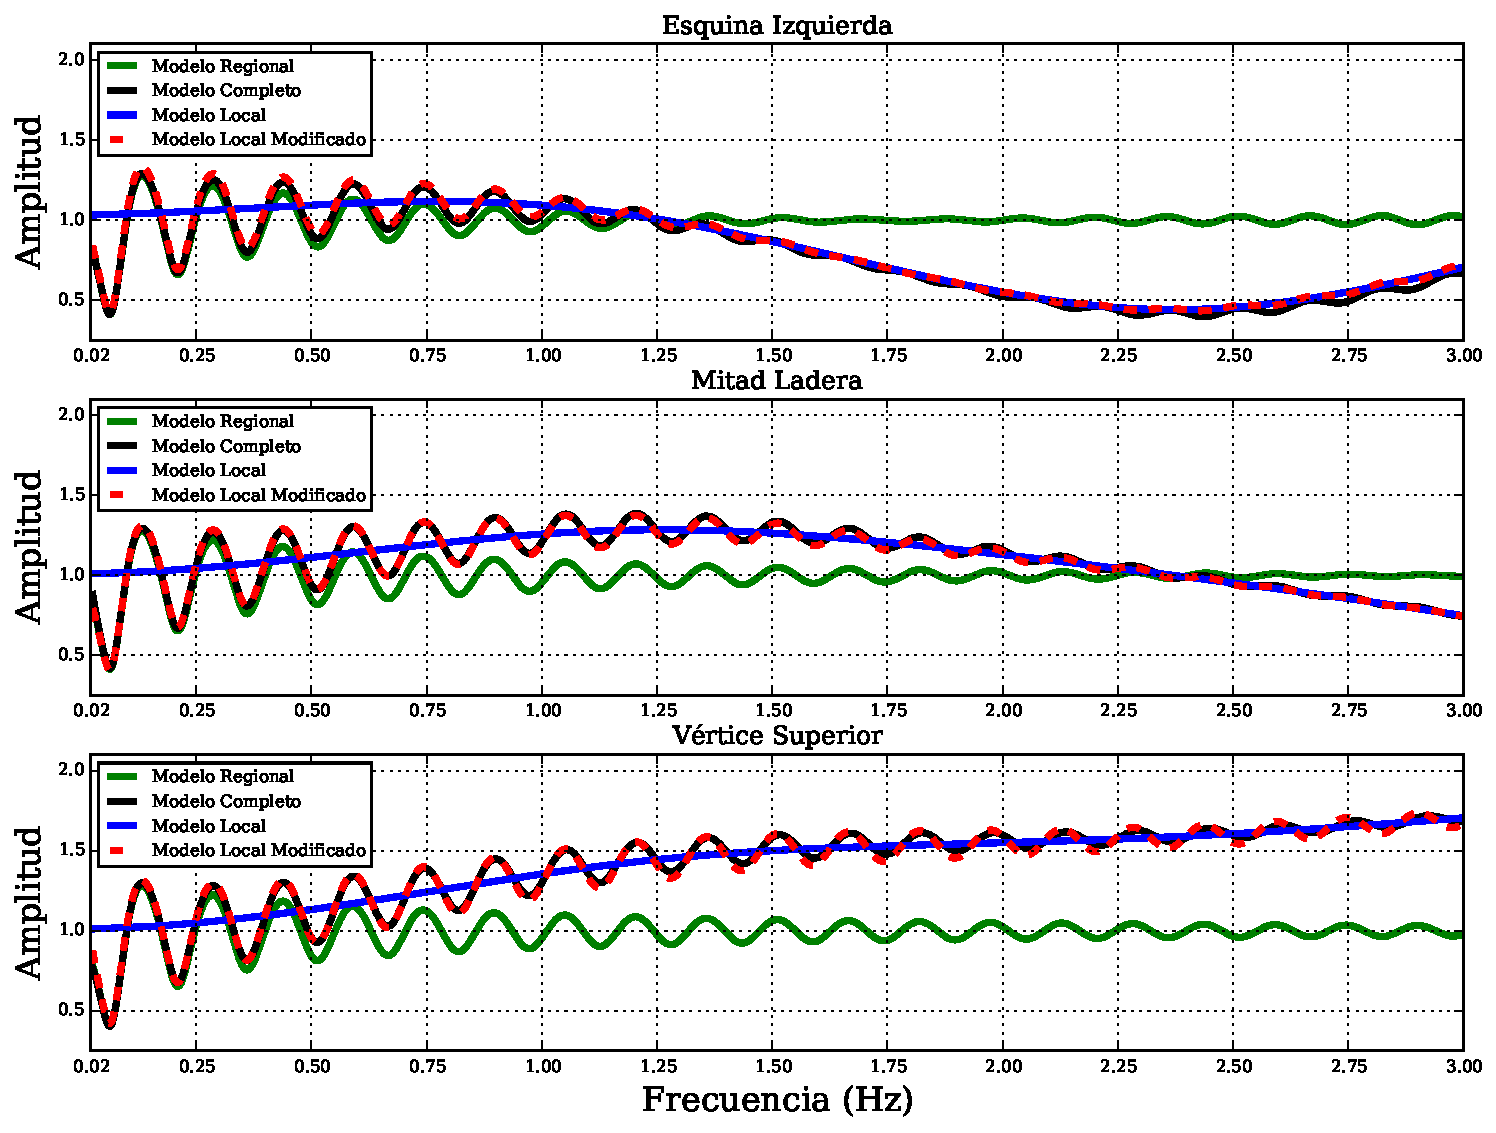
\includegraphics[width=15 cm]{img/TransFuncHom.pdf}
	\vspace{-.5 cm}
	\caption{Funciones de Transferencia Modelos Homogéneos}
	\label{fig:tfhom}
	\vspace{-1 cm}
\end{figure}
%
%
%
%
%
\subsection{Montaña Triangular Embebida en un Sector Semi-Circular, Modelo In-Homogéneo}
%
Para el semiespacio se define una velocidad de propagación de onda de corte $\beta_{HS} = 1.00\ km/s$, la del dispersor tipo montaña se define igual a la mitad de la del semi espacio $\beta_{Dispersor} = 0.50\ km/s$, se emplea la misma densidad $\rho = 1000\ kg/m^3$ para los materiales presentes en el dominio y se usa una frecuencia máxima $f_{max} =  16\ Hz$. Al igual que en el caso anterior, el sector semicircular tiene un radio $r=2.50\ km$, la montaña tiene una base $b=0.30\ km$ y altura $h=0.10\ km$.

Para los tres modelos se emplean $12$ puntos por longitud de onda $\left( p = 12 \right)$ para mantener la misma cantidad de elementos del caso anterior.

En la \cref{fig:ftspatialIn} se muestran las funciones de transferencia sobre la superficie de los tres modelos de la \cref{fig:model1}, entre las coordenadas $-0.15\ km$ y $+0.15\ km$.\\
%
En la \cref{fig:ftspatialIn}a al igual que en la \cref{fig:ftspatial}, no se observa variación espacial de la respuesta. La respuesta del modelo local de la figura \ref{fig:model1}b tiende a la de un semiespacio dado que la longitud de onda es aproximadamente $8$ veces el ancho de la base de la montaña la cual es bastante grande, $\lambda= 2.50\ km$, y la respuesta no ve el dispersor; por ésta misma razón, la respuesta del modelo regional y la del modelo completo son casi iguales.
%
\begin{figure}[H]
	\centering
	\subfloat []{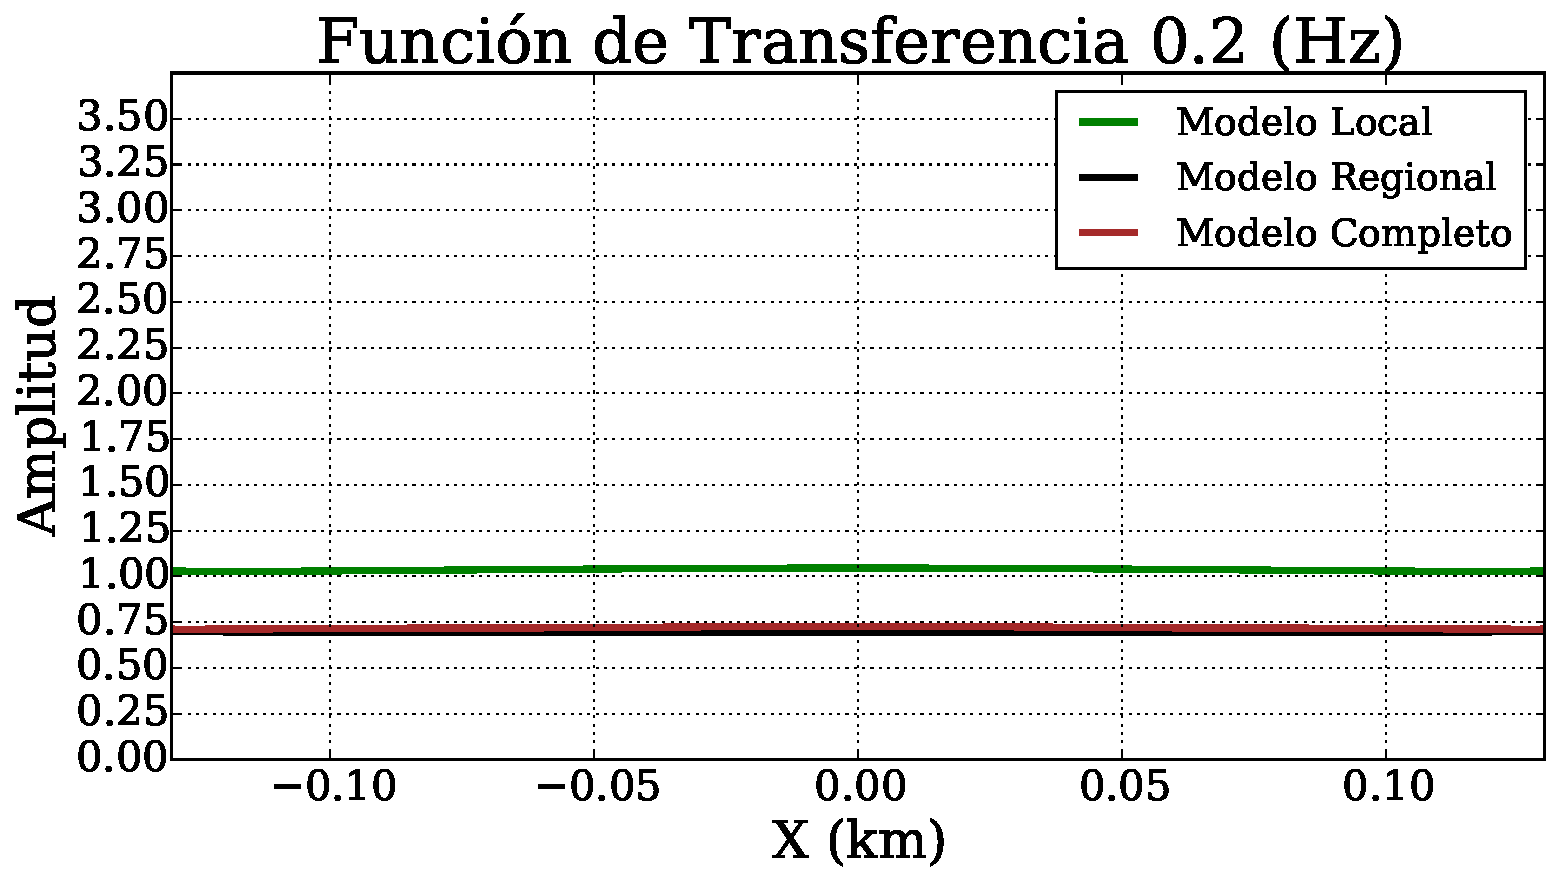
\includegraphics[width=8 cm]{img/TF_InHomogeneo_2.pdf}}
	\subfloat []{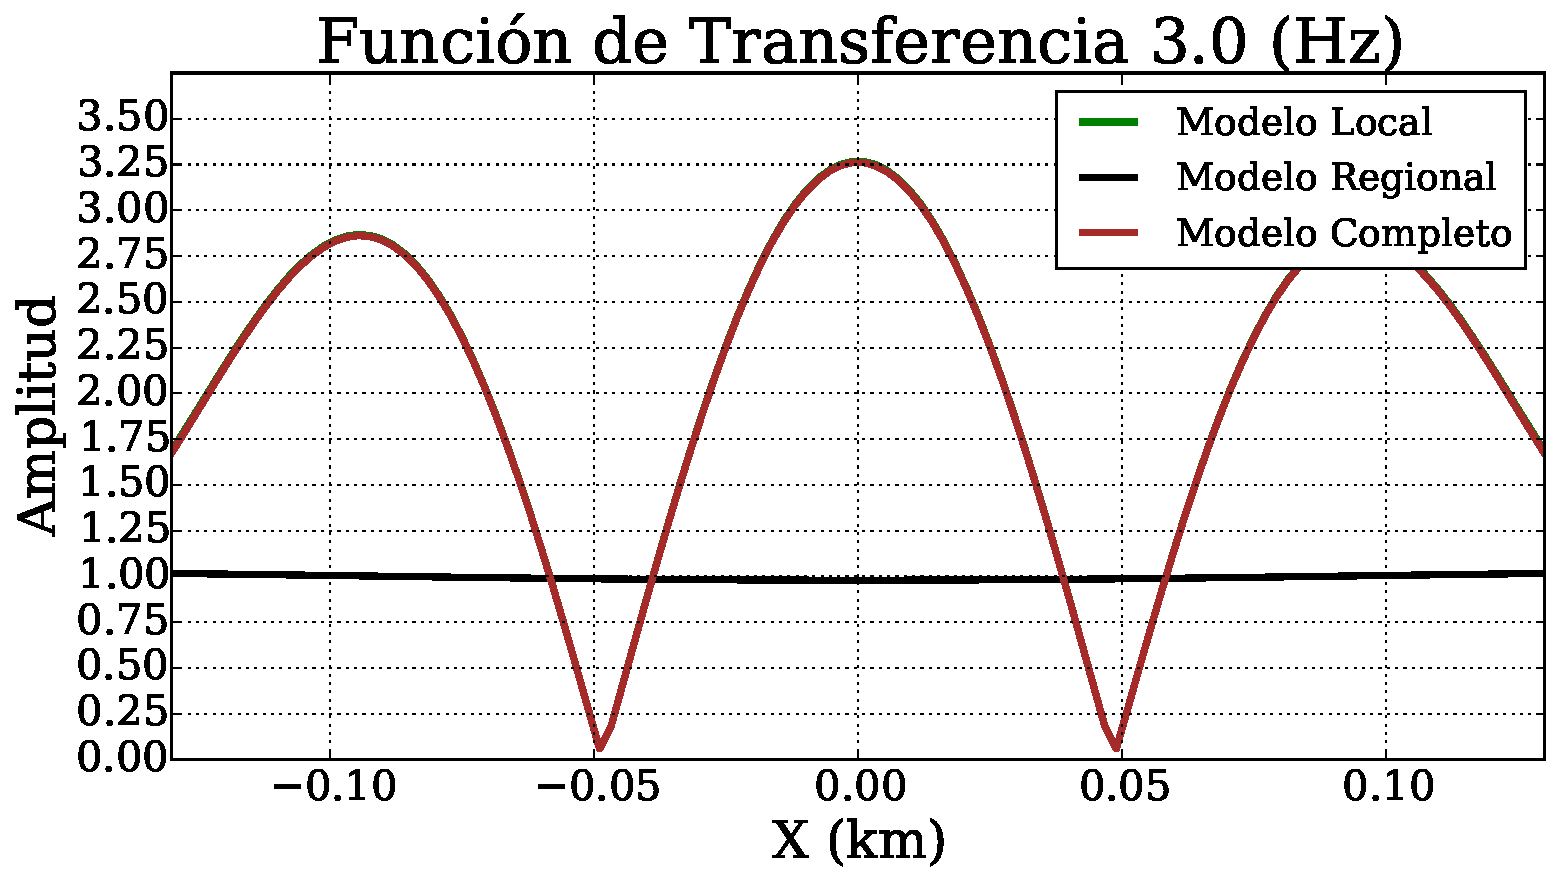
\includegraphics[width=8 cm]{img/TF_InHomogeneo_30.pdf}}\\
	\vspace{-.5 cm}
	%
    \caption{Funciones de Transferencia Espaciales Modelos InHomogéneos.}
    \label{fig:ftspatialIn}
    \vspace{-1 cm}
\end{figure}
%
En la \cref{fig:ftspatialIn}b se observa una variación espacial mucho mayor a la de la \cref{fig:ftspatial}b debido a que en éste modelo la longitud de onda es aproximadamente igual a la mitad de la base de la montaña, $\lambda = 0.167\ km$. Como en ésta figura se muestra la amplitud de la función de transferencia, la distancia entre dos picos consecutivos corresponde a la mitad de la longitud de onda, por lo tanto a medida que aumenta la frecuencia se presenta una mayor variación espacial de la respuesta.

En la \cref{fig:tfinhom} se muestran la funciones de transferencia sobre las tres ubicaciones de la superficie de los modelos analizados, ver \cref{fig:puntos}. 

De ésta figura se pueden sacar las mismas conclusiones del modelo anterior, lo cual indica que el método funciona bastante bien aún en presencia de efecto acoplado suelo topografía.

\begin{figure}[H]
	\centering
	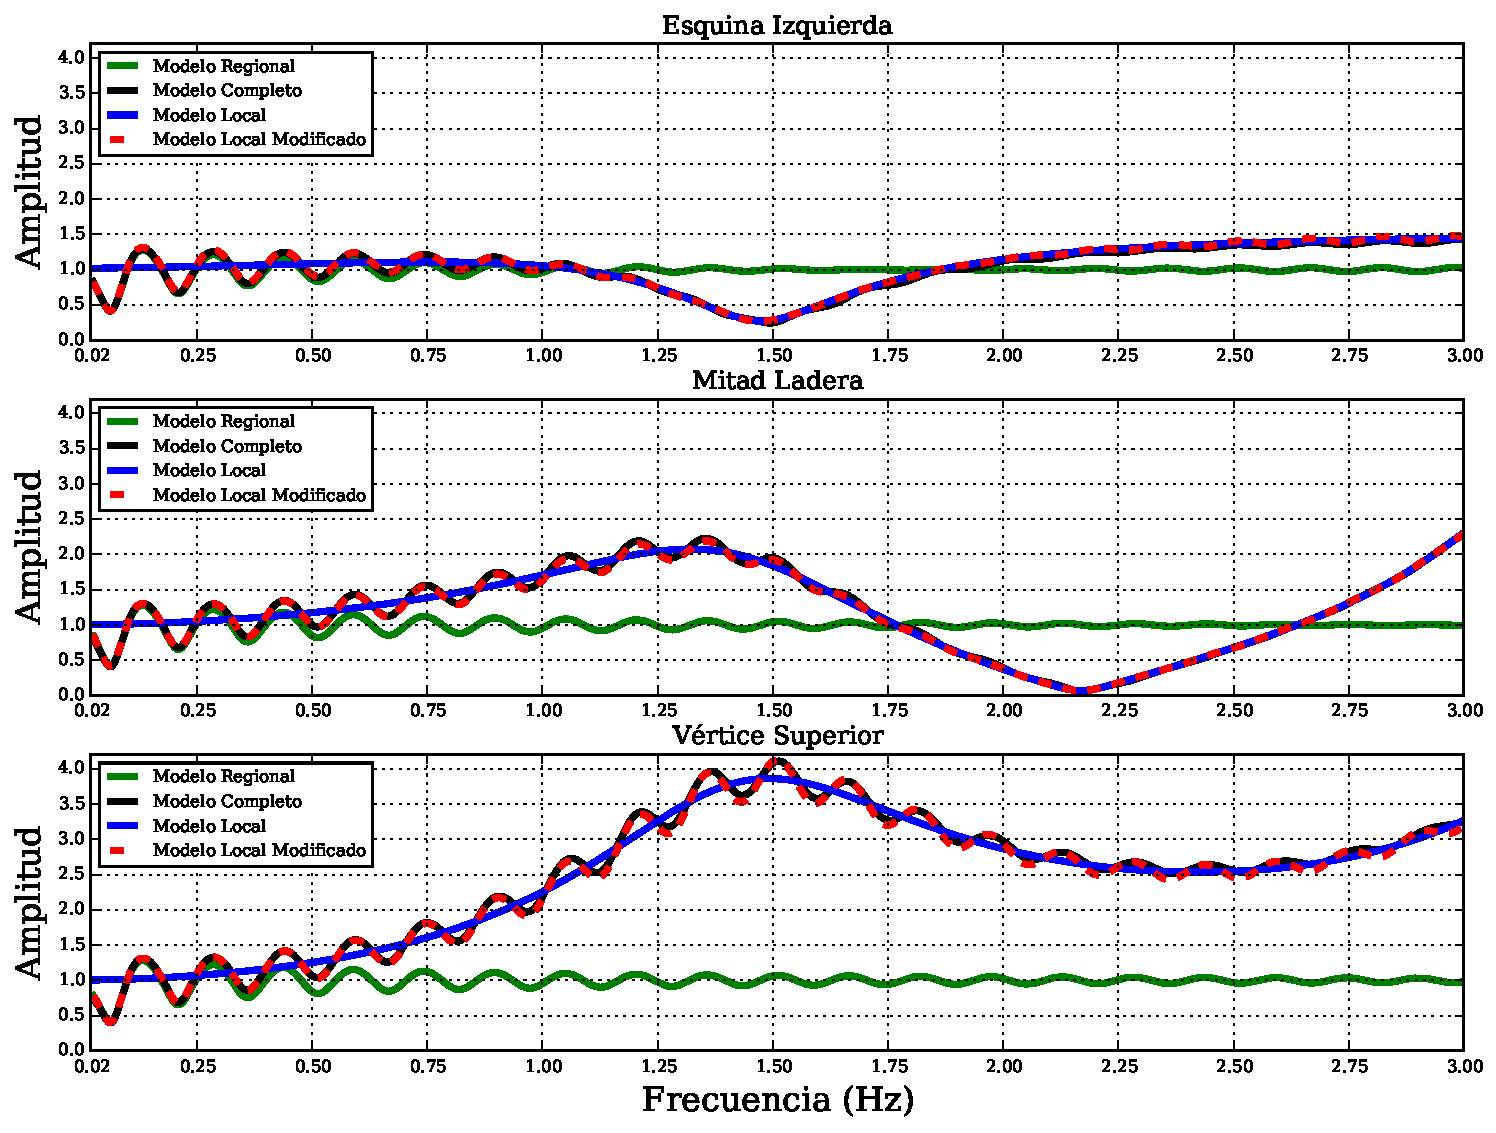
\includegraphics[width=15 cm]{img/TransFuncInHom.pdf}
	\vspace{-.5 cm}
	\caption{Funciones de Transferencia Modelos InHomogéneos}
	\label{fig:tfinhom}
	\vspace{-1 cm}
\end{figure}
%
%
%
%
%
\bibliographystyle{gji}
\bibliography{refproposal}


\end{document}
